\documentclass[english]{article}
\usepackage[T1]{fontenc}
\usepackage[utf8]{inputenc}

\usepackage{babel}
\usepackage{authblk}
\usepackage{xspace}
\usepackage{diagbox}
\usepackage{graphicx,graphics} 
\usepackage{color}
\usepackage{amsmath}
\usepackage{amsfonts}
\usepackage{caption}
\usepackage{algorithm}
\usepackage{algorithmic}
\usepackage{amssymb}
\usepackage{amsthm}
\usepackage{algorithm}
\usepackage{algorithmic}
\usepackage{longtable}
\usepackage{complexity}
\usepackage{hyperref}
\usepackage{tkz-graph}
\begin{document}

\title{ Deterministic Scheduling to Minimize Latency in Meshed Networks}
 

\newcommand{\todo}[1]{{\color{red} TODO: {#1}}}
\newcommand{\spall}{\textsc{SPALL}\xspace}
\newcommand{\bra}{\textsc{BRA}\xspace}
\newcommand{\ADO}{\textsc{ADO}\xspace}
\newcommand\greedydeadline{\texttt{Greedy Deadline}\xspace}
\newcommand\greedynormalized{\texttt{Greedy Normalized}\xspace}
\newcommand\greedypacked{\texttt{Greedy Packed}\xspace}
\newcommand\hybridgreedydeadline{\texttt{Hybrid Greedy Deadline}\xspace}
\newcommand\hybridgreedynormalized{\texttt{Hybrid Greedy Normalized}\xspace}
\newtheorem{theorem}{Theorem}
\newtheorem{lemma}[theorem]{Lemma}
\newtheorem{proposition}[theorem]{Proposition}
\newtheorem{corollary}[theorem]{Corollary}
\newtheorem{definition}{Definition}

\author[1]{\bf{ {Dominique Barth}}}
\author[1,2]{\bf{ {Ma\"el Guiraud}}}
\author[2]{\bf{ {Brice Leclerc}}}
\author[2]{\bf{ {Olivier Marc\'e}}}
\author[1]{\bf{ {Yann Strozecki}}}


\affil[1]{David Laboratory, UVSQ}
\affil[2]{Nokia Bell Labs France}


\maketitle

\section{Introduction}

TODO: doner le contexte CRAN, puis l'objectif d'optimisation de latence. 
Dire qu'on a déjà fait désynchronisé mais que dans les architectures actuelles il faut plutot faire synchronisé.
Comparer à nos travaux antérieurs et à d'autres qu'on a déjà cité (voir les papiers précédents, surtout les citations du dernier).




\section{Scheduling of Periodic Datagrams over a Network: the problem \spall}


Let $[n]$ denote the interval of $n$ integers $\{0,\dots,n-1\}$.

  \subsection{Modeling the Network and its Contention Points}

  We study a communication network with pairs of source-destination nodes between which messages are sent periodically. The routing between each  pair of such nodes is given. The network is represented by a directed acyclic multigraph $G=(V,A)$. The set of vertices is composed of three disjoint subsets:  ${\cal S}$ the set of sources of the messages, ${\cal D}$ the set of destination of the messages, and ${\cal C}$ the set of contention points in the network. Indeed, some links of the network are shared between several pairs of source-destination nodes. A contention point represents the beginning of a shared link, i.e. the physical node of the network which sends the messages into the link. An arc in $G$ can represent several physical links or nodes, which do not induce contention points. Each arc  $(u,v)$ in $A$ is labeled by an integer weight $\omega(u,v)$ which represents the time elapsed between the sending time of the message in $u$ and the reception time of this message in $v$ using this arc. \\
  A {\bf route} $r$ in $G$ is a directed path, that is, a sequence of adjacent vertices $u_1, \ldots , u_{l}$, with $(u_i,u_{i+1}) \in A$.  The {\bf weight of a vertex} $u_i$ in a route $r=(u_0,\dots,u_l)$ is defined by $\lambda(u_i,r)= \sum\limits_{1 \leq j <i} \omega(u_j, u_{j+1})$. It is the number of tics needed by a message to go from the first vertex of the route to $u_i$. The \textbf{length} of the route $r$ is defined by $\lambda (r)= \lambda (u_l,r)$.
	We denote by ${\cal R}$ a set of routes of the graph $G$, the pair $(G,{\cal R})$ is called a \textbf{routed network} and represents our telecommunication network.\\
	Let $r \in {\cal R}$, with $r = (u_0,u_1,\dots,u_l)$, then we say that $u_i$ is of \textbf{contention level} $i$ for the route $r$, and we denote it by $cl(u_i,r) = i$. The contention level of a node $u$ is the maximum of its contention level over all routes going through itself: 
	$cl(u) = \max\limits_{r\in{\cal R} \text{ and } u \in r} cl(u,r)$.

\begin{figure}

\begin{minipage}[c]{.45\linewidth}
	
	
	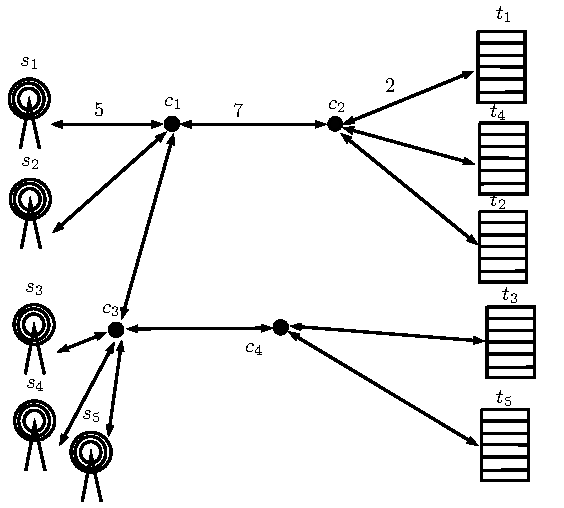
\includegraphics[scale=0.5]{fronthaul}



	 \end{minipage} 
 \hfill
 \begin{minipage}[c]{.45\linewidth}
	
	
	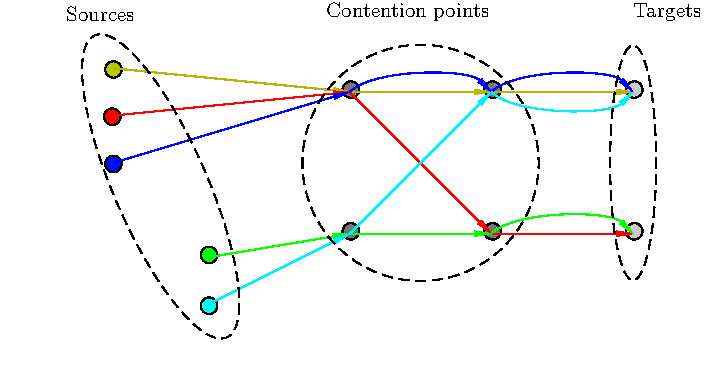
\includegraphics[scale=0.5]{graphmodel}\\

	 \end{minipage}
	 
\caption{A C-RAN fronthaul network and its corresponding routed network}
\label{fig:fronthaul}
\end{figure} 
	The  \textbf{contention depth} of a routed network $(G,{\cal R})$ is equal to the maximum of the contention level over all vertices. It is the number of contention points on the longest route of the network. In all the article, $(G,{\cal R})$ is the routed network, ${\cal C}$ is the set of its contention vertices, $n$ denotes $|\cal{R}|$ the number of routes and $d$ is the contention depth.  


 \subsection{Dynamic of Datagrams Transmissions}
	    
 		In this article, we consider a discretized time. The unit of time is called a {\bf tic}. This is the time needed to send an atomic data in a link of the network. We assume that the speed of the links is the same over all the network. Several of the authors are developing a prototype based on ethernet base-X~\cite{ieee_8023}, using standard values for the parameters of the network: the size of an atomic data is $64$ bits, the speed of the links is $10$Gbps, and the length of a tic is thus about $6.4$ nanoseconds. 

        In the process we study, a message called a {\bf datagram} is sent on each route from the source node. The \textbf{size} of a datagram is an integer, denoted by $\tau$, it is the number of tics needed by a node to emit the full datagram through a link.  In this paper, we assume that $\tau$ is the same for all routes. It is justified by our application to C-RAN, where all source nodes are RRHs sending the same type of message. There is no preemption: Once a datagram has been emitted, it cannot be fragmented during its travel in the network. We assume that the first datagram sent on each route is available at time $0$.

          Let $r=(u_0,\dots,u_l)$ be a route. In order to avoid contention, it is possible to buffer datagrams in contention points. The function $A$, called an \textbf{assignment}, associates an integer value, greater or equal to $0$, to each couple (route,vertex) of the routed network $(G,{\cal R})$. Those integers represent the buffering time of the datagrams in the nodes of the network: a datagram of route $r$ waits $A(r,u)$ tics in the buffer of vertex $u$.
          
       

 The \textbf{arrival time} of a datagram in vertex $u_i$ of $r$, is the first time at which the datagram sent on $r$ reaches $u_i$, and is defined by $t(r,u_i) = \lambda(u_i,r) + \sum_{k=0}^{i-1} A(r,u_k) $. The date at which a datagram reaches a vertex $u_i$ is decomposed into a \emph{physical delay} due to the time to go through the links before $u_i$ and a \emph{logical} delay caused by the use of buffers as determined by assignment $A$.
  The \textbf{sending time} of a datagram at vertex $u_i$ of $r$, is the first time at which the datagram is sent by $u_i$. It is defined by $s(r,u_i) = t(r,u_i) +  A(r,u_i) $. This is the arrival time of the datagram plus the buffer time given by $A$.
 
  If $u_l$ is the last vertex of the route $r$, the transmission time of the datagram on 
  $r$ is denoted by $TR(A,r)$ and is equal to $t(r,u_l)$. We define the \textbf{transmission time} of an assignment $A$ as $TR(A) = \displaystyle \max\limits_{r \in {\cal R}} TR(A,r) $. This is the time elapsed before the reception of the beginning of the last datagram. 
%   In the application we study the full transmission time is bounded . We define $Tmax$ such that $TR(A) \leq Tmax$.
         
  \subsection{From C-RAN Networks to Routed Networks}
  \label{subsection:CRANGRAPH}

  This study is motivated by a problem arising from Cloud RAN: messages containing local radio information are sent by a radio antena (called RRH) to a BaseBand Unit (BBU) in a datacenter through a fronthaul network. Then, the datacenter sends back an answer to the RRH. The routed network presented in this article is used to modelize both ways of this communication, from an RRH to the corresponding BBU and back to the RRH. Hence, each RRH corresponds to the first and the last vertex of a route. The BBU is not a node of the routed network, since each RRH has its own BBU, there are no contention when going through the BBU. The datagram arrives at the BBU somewhere on an arc of the route. Once a datagram arrives at its BBU, the answer is computed and sent back over the fronthaul network. The computation time is usually the same for all messages; it is encoded into the arc corresponding to the BBU by adding it to the physical delay of transmission over the arc.
  
  In this article, we consider that the links of the fronthaul network are full duplex, that is the messages can go through the links in both ways, without interacting. Usually the route from the RRH to the BBU is the same (with the orientation reversed) as the route from the BBU to the RRH. This property does not need to be enforced in our theoritical modeling, but it matches real fronthaul network and we will use such examples for our experiments. 

  %Remark that the routed network induced by such topologies are symmetric. Pas vraiment
  
    Several BBUs are gathered in one or several datacenters. The length of the links between the entrance of the datacenter and all BBUs may or may not be the same. In the first case, once the messages have been scheduled to go in the datacenter, they go out in the exact same order and thus, even if all routes use the same link in the way back, it is not considerd as a contention point, as illustrated in figure~\ref{fig:allerretour}. If the length of the links into some datacenter are different, the contention point before the datacenter is also a contention point at the exit of the datacenter and the routes are symmetrical around this vertex.

    \begin{figure}

	\centering
	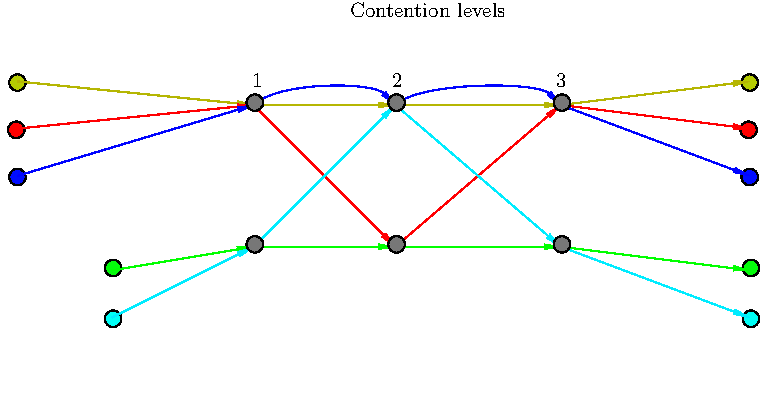
\includegraphics[scale=0.8]{allerretour}


\caption{The routed network modeling datagrams going back and forth in the fronthaul network of figure~\ref{fig:fronthaul}.}
\label{fig:allerretour}
\end{figure}

Finally, the fronthaul networks we study have \textbf{coherent} routings, a classical 
requirement in telecommunication networks (see e.g. ~\cite{schwiebert1996necessary}). It means that
if the routes $r$ and $r'$ go through two contention points $u$ and $v$, they have the same subpath
between $u$ and $v$.
This is true for the fronthaul networks we modelize. Hence in the routed network which represents 
going back and forth in the fronthaul network, the coherent property is respected from the source 
to the arc representing the BBU and then form the arc representing the BBU to the target.
 As a consequence, routed networks obtained from fronthaul networks are directed acyclic multigraphs, as required in the definition of routed network.
     
  \subsection{Periodic Emission of Datagrams}

 	The process we model in this article is \emph{periodic}: for each period of $P$ tics, a datagram is ready to be sent from each source node in the network at time zero of the period. The process is assumed to be infinite, since it should work for an arbitrary number of periods. We chose to always use the same buffering in all periods, for simplicity of implementation in real networks but also to make our problem more tractable from a theoritical perspective. In other words, at the same time of two different periods, all messages are at the same position in the network: the assignments we build are themselves periodic of period $P$. Thus, we only need to consider the behavior of the datagrams on each node of the network during a single period, and to apply the same pattern to every subsequent period. 
    Let us call $[r,u]_{P,\tau}$ the set of tics used by a datagram on $r$ at vertex $u$ in a period $P$, that is $[r,u]_{P,\tau} = \{s(r,u) + i \mod P \mid 0 \leq i < \tau \}$. 

      Let us consider two routes $r_1$ and $r_2$, they have a {\bf collision} at the contention point $u$ if and only if $[r_1,u]_{P,\tau} \cap [r_2,u]_{P,\tau} \neq \emptyset$.\\

        An assignment $A$ of a routed network $(G,{\cal R})$ is said to be \textbf{valid} if \emph{no pair of routes has a collision}. 
        The validity of an assignment depends on $P$ the period and $\tau$ the size of the messages, but in this article these values are fixed and they are not made explicit in the assignment (contrarily to previous work~\cite{Guir1806:Deterministic}).
        Note that the period $P$, as well as the size of a message $\tau$ is fixed in our $C-RAN$ application, but not the buffering policy. Hence, the aim of our work is to find a valid assignment which minimizes the latency of transmissions over the network, that is $TR(A)$.
       \\ 
       
       \noindent {\bf Synchronized Periodic Assignment for Low Latency (\spall)} 

      \noindent {\bf Input:}  Symmetric routed network $(G,{\cal R})$, period $P$, datagram size $\tau$.%, a bound on the latency $T$.
      
      %\noindent {\bf Decision problem:} is there a valid assignment $A$ of $(G,{\cal R})$ such that $ TR(A) \leq T$ ?

      \noindent {\bf Output:} assignment $A$ which minimizes $TR(A)$.
      \\
    
    Several parameters are important for the study of \spall. The algorithms we present have a complexity
    depending on $n$ the number of routes and $d$ the contention level. We evaluate the arithmetic complexity of our algorithms, that is arithmetic operations are considered to be in constant time. Then, the complexity will surprisingly not depend on $P$, $\tau$ or the weights of the routed network.
    Given a contention point $u$, let ${\cal R}_u \subseteq {\cal R}$ be the set of routes which contain $u$. The \textbf{load} of $u$ is $\tau|{\cal R}_u|/P$, it measures the percentage of the bandwidth used by datagrams going through $u$. The load of $(G,{\cal R})$ is the maximum of the load of $u$, for all contention vertices in $G$.
    This parameter is crucial in the theoritical study of a simpler variant of \spall~\cite{guiraud2020scheduling}, and is also important to the practical performance of algorithms presented in this article.


\subsection{Contention Depth and \spall}
\label{sec:contentiondepth}
\paragraph*{Contention Depth One}

Each contention vertex of a routed network of contention depth one induces a connected component. 
Problem \spall can be independently solved on each connected component, hence the case with a single contention point is equivalent to contention depth one. 
If we remove the periodicity from \spall on a single contention point, it can be seen as a single processor scheduling problem, where datagrams are jobs of the same size, their release times are given by the length of the arc to the contention point, and the deadline of each job is computed from the length of the route.
The scheduling problem is as follows: each job must be scheduled such that no two jobs uses the machine at the same time. Each job must be scheduled after its release time and must satisfy its deadline. The makespan of a solution is the time elapsed between the beginning of the computation of the first job and the end of the last job. There is a polynomial time algorithms to find a scheduling that minimizes the makespan~\cite{simons_fast_1978}.

Solving the same problem, but taking into account periodicity is solving \spall over 
a routed network with a single contention point. This problem has already been defined and studied in~\cite{barth2018deterministic} under the name \bra. We proved that it can be solved by reducing it to at most 
$2^n$ instances (much less in practice) of the non periodic variant. 
While $\bra$ may be in $\P$, when messages have different sizes, the non periodic scheduling problem is known to be $\NP$-hard~\cite{}. It implies $\NP$-hardness for \bra with different message sizes, since the periodic problem is equivalent to the non-periodic one by taking a large enough period, say the maximum of the lengths of the routes plus the number of routes times $\tau$.



     
%\noindent{\bf \bra} 

%      \noindent {\bf Input:} A routed network of depth one $(G,{\cal R})$, the size of the messages $\tau$, a period $P$.\\
%      \noindent {\bf Question:} Find an assignment of  $(G,{\cal R})$ that minimizes $TR(A)$.\\

   
 %  \begin{theorem}\label{th:braFPT}
%$\bra \in \FPT$ when parametrized by the number of routes.
%\end{theorem}
%   The proof of this theorem is explained in~\cite{barth2018deterministic}. It is possible that \bra is solvable in polynomial time, but we did not investigate this point enought yet.
   


We can further restrict the problem, by asking that all weigths of arcs from sources to the contention point
are the same or equivalently all weigths from the contention point to the destination are the same. 
Then, it is enough to consider all datagrams and their time of avalabality in the contention point ...
\todo{décrire proprement l'algo greedy GD qui marche ici, puisqu'on s'en sert pas mal après} 

\paragraph*{Star Shaped Network}

The most simple case of contention depth $2$ is a routed network with two contention points. 
This is enough to modelize our process of sending a datagram from an RRH to a BBU and back when
there is a single contention point (a shared link between the RRHs and the data centers). 
This topology, called \emph{star shaped network} in previous work, is classical in fronthaul networks, and a non synchronized version of \spall has been studied on star shaped networks~\cite{Guir1806:Deterministic,barth2018deterministic,guiraud2020scheduling}.


 \begin{theorem}\label{th:braFPT}
The problem $\spall$ on star shaped network is $\NP$-hard
\end{theorem}
\begin{proof}
The two flow shop problem studied in~\cite{yu2004minimizing} is shown to be $\NP$-hard. The problem is as follows, a set of jobs have to be processed in sequence on two machines; a job must be processed on machine $1$ before beeing processed on machine $2$. There is, for each job, a delay between the end of the processing on the first machine and the begining of the processing on the second one. The objective is to minimize the makespan. The time needed to process each job is the same.\\
We reduce an instance of $\spall$ in an instance of the two flow shop proplem: A message is a job, the delay of the jobs are equivalent to the lenght of the routes between the two contention points. We then set the makespan value to $P$, and the instance of $\spall$ becomes an instance of two flow shop.
\end{proof}


\paragraph*{Contention Depth Two and More}

However, star shaped networks may not be the most general topology with regard to problem \spall.
Que peut-on dire des topologies de profondeur 2 en général ? Expliquer que si elles modélisent un aller-retour,
ce sont forcément des star shaped networks.
Introduire les réseaux plus généraux de contention depth 3.Dire comment ce qu'on veut modéliser est un cas particulier de
contention depth 3: profondeur 2 dans le réseau, même
distance de tous les datacenters dans les BBUs ce qui vire un point de contention. Donner un exemple illustré.
   \begin{figure}

	\centering
	\includegraphics[scale=0.8]{bbuaggreg}


\caption{One or several contention points around the BBU according to the lenght of the links}
\label{fig:allerretour}
\end{figure}


\section{Compact Representation of an Assignment}

 We define $\prec$, the pointwise order on assignments: $A_1 \preceq A_2$ if for all $r\in \cal{R}$, $TR(A_1,r) \leq TR(A_2,r)$. Moreover, we say that $A_1 \prec A_2$ if $A_1 \preceq A_2$ and there is an $r \in \cal {R}$ such that  $TR(A_1,r) < TR(A_2,r)$. Remark that assignments which minimize $TR(A)$ are also minimal for $\prec$. Hence, it is enough to consider minimal assignments for $\prec$ to solve \spall.

We explain in this section how to represent most assignment in a compact way, forgetting about the precise buffering time by only considering informations about the order of the datagrams in each contention point. All minimimal assignments have a compact representation, which implies that we do not need to consider assignment without a compact representation when solving \spall. 
It allows to design an FPT algorithm for \spall by going through all compact representations, but also to design good polynomial time heuristics using taboo search or simulated annealing, since one can easily define the neighborood of a compact representation.


\begin{definition}[Compact assignment]
Let $(G, \mathcal{R})$ be a routed network. A compact assignment $CA$ is a function which maps to each contention point $u$ in $G$ a pair $(O_u,S_u)$, where $O_u$ is an order on $R_u$ and $S_u$ is a subset of $R_u$.
\label{definition:compact}
\end{definition}


\subsection{From a Valid Assignment to its Compact Representation}

Let us define a function which maps a valid assignment $A$ to a compact assignment, called the compact representation of $A$, denoted by $CR(A)$. Let assume that for all contention vertices $u$, there is a route $r \in \mathcal{R}_u$ such that $A(r,u) = 0$.

We assume that routes in $\mathcal{R}$ are indexed by the integers in $[n]$. Say w.l.o.g. that $r_0$ is the route of smallest index such that $A(r_0,u) = 0$. The datagram of $r_0$ arrives, and goes to the next contention vertex, at time $t(r_0,u)$. Let us define the \textbf{normalized arrival time} of $r$ at $u$: for all $r \in \mathcal{R}_u$, $nt(r_0,r,u) = (t(r,u) - t(r_0,u)) \mod P$. It is the time at which the datagram of $r$ arrives at $u$, in a period normalized so that the datagram of $r_0$ goes through $u$ at time $0$. Similarly, we define the \textbf{normalized sending time} as $ns(r_0,r,u) = (s(r,u) - t(r_0,u)) \mod P$.

We define $O_u$ as the order on the routes of $R_u$ induced by the values $ns(r,u)$. The set $S_u$ is defined as the set of routes going through $u$ such that $ns(r_0,r,u) < nt(r_0,r,u)$. Represent the time as cut into periods $[t(r_0,u) + iP,t(r_0,u) + (i+1)P [$ with $i \in \mathbb{N}$. Intuitively, $S_u$ represents the set of routes with a datagram going through $u$ in the period \emph{after} the one it has been available in. 

Fig.~\ref{fig:normalizedassignment} illustrates how a compact representation is computed from an assignment on a single node $u$. On top, the datagrams are represented by sending time $s(r_i,u)$ while the bottom of the figure shows the datagrams in a single period, represented by normalized sending times $ns(r_0,r_i,u)$.  
\begin{figure}[!h]
	\centering
	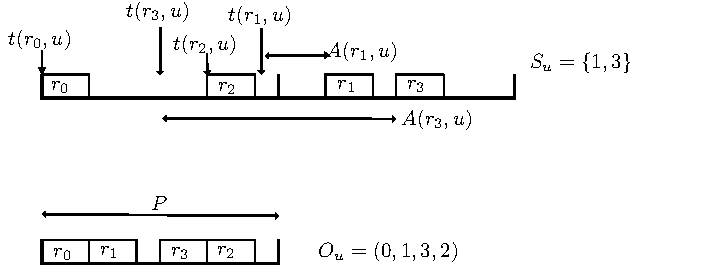
\includegraphics[scale=1]{normalizedassignment}
\caption{A compact representation of an assignment in which $O_u = (0,1,3,2)$ and $S_u = \{1,3\}$ }
\label{fig:normalizedassignment}
\end{figure}


Note that for $CR(A)$ to be defined, we need that, on each contention point, at least a datagram is not buffered. We call such an assignment a \textbf{canonical assignment}. It turns out that any assignment $A$ can be made canonical without increasing $TR(A)$.

\begin{lemma}\label{lemma:canonical_min}
Let $A$ be a valid assignment, then there is a valid canonical assignment $A'$ such that $A' \preceq A$.
\end{lemma}
\begin{proof}
Consider a vertex $u$ of contention level $1$, such that for all $r \in \mathcal{R}_u$, $A(r,u) > 0$. Let us define $m$ as the minimum of these values, we define $A'(r,u) = A(r,u) - m$. Assignment $A'$ has no collision on $u$, since all departure times have been shifted by the same value and $A$ has no collision. Moreover, if $v$ is the vertex after $u$ in a route $r$, we define  $A'(r,v) = A(r,v) + m$. Hence, all departure times for vertices of contention levels larger than one are the same in $A$ and $A'$, which implies that there are no collisions in these vertices. We have proven that $A'$ is still valid. Since all departure times of $A'$ are less or equal to those induced by $A$, we have $A' \preceq A$. Moreover, if $r_0$ is the route with $A(r_0,u) = m$, then $A'(r_0,u) = 0$. 

We apply this transformation by increasing contention level. Since, the transformation applied at some contention level do not change $A'$ for smaller contention levels, a trivial induction proves that $A'$ is valid, canonical and that $A' \preceq A$.
\end{proof}


\subsection{From a Compact Assignment to its Realization}


We now explain how to transform a compact representation into a canonical assignment.
Moreover, we show that the obtained assignment is the smallest among all assignments of same representation. We first explain how to do the transformation on a routed network with a single contention vertex $u$.

Recall that the datagram of a route $r$ is available at time $t(r,u)$ in the vertex $u$.
Let us consider a compact assignment $CA$, which maps $u$ to the pair $(O_u,S_u)$.
The assignment $Real(CA)$ is built inductively from $CA$, it is called the realization of $CA$. 
If the construction of $Real(CA)$ fails, then $Real(CA)$ is undefined and we say that $CA$ is not realizable. In the next paragraph, we build an assignment $A$ by setting the buffering time of the routes in the order
 $(O_u)$. If the construction suceeds, we set $Real(CA) = A$ 

Let say that the order $O_u$ is $(r_0, \dots, r_l)$. We fix $A(r_0,u)$ to zero, that is the first
datagram in the period has no buffering time. Then, in each period beginning by the first datagram, the datagrams will be in order $O_u$. When the first datagram of the period is chosen, we use it to define normalized arrival times and normalized sending times.
Assume that $A(r_i,u)$ have been set for $i \leq l$, let us explain how to 
set $A(r_{i+1},u)$. If $r_{i+1} \notin S_u$, then $A(r_{i+1},u)$ is chosen so that $ns(r_1,r_{i+1},u)$ is the maximum of $ns(r_1,r_i,u) + \tau$ and $nt(r_1,r_{i+1},u)$. If $ns(r_1,r_{i+1},u) > P - \tau$, then $CA$ is not realizable. If $r_{i+1} \in S_u$, then $A(r_{i+1},u)$ is chosen so that $ns(r_1, r_{i+1},u) = ns(r_1,r_i,u) + \tau$. In both cases, if $ns(r_1, r_{i+1},u) \geq nt(r_1,r_{i+1},u)$, then $CA$ is not realizable (the sending time is in the wrong period with regard to $S_u$). 

Figure~\ref{fig:compacttoassignment} shows how an assignment $Real(CA)$ is built from a compact assignment $CA$ on a single contention vertex $u$. We have $O_u = (2,1,0,3)$ and $S_u = \{1\}$. First, the datagram $2$ is fixed, that is, $A(r_2,u)=0$. Then, since $r_1 \in S_u$, we set $A(r_1,u)$ such that $ ns(r_2,r_1,u) = ns(r_2,r_2,u) + \tau$. 
Finally, since $r_0$ and $r_3 \notin S_u$, we set $A(r_0,u)$ and $A(r_3,u)$ such that $ns(r_2,r_0,u) = nt(r_2,r_0,u)$ and  $ns(r_2,r_3,u) = ns(r_2,r_0,u) + \tau$.
\begin{figure}[!h]
	\centering
	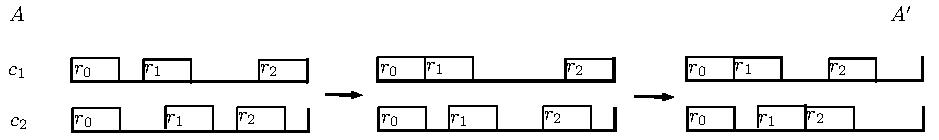
\includegraphics[scale=1]{compacttoassignment}
\caption{Inductive construction of $Real((2,1,0,3),\{1\})$ from $CA$ on a single contention vertex $u$. }
\label{fig:compacttoassignment} 
\end{figure}

The function $Real$ can easily be generalized to any routed network. Indeed, one can first consider all vertices of contention level $1$, the routes going through them form disjoint sets. Hence, we can define $Real$ independently on each vertex of contention level $1$. 
Then using the buffering computed for this vertices, one can compute the arrival time of each route in vertices of contention level $2$ and compute $Real$ for these vertices in the exact same way, and so on for all contention levels. In the following lemmas and theorems, we always consider a single contention vertex, since it is trivial to extend any property for one contention vertex to the whole routed network as we just explained. 

\begin{lemma}\label{lemma:canonical}
The assignment $Real(CA)$ can be computed in time $O(nd)$, where $d$ is the contention
depth of the network. If $CA$ is realizable, then $Real(CA)$ is a valid canonical assignment.
\end{lemma}
\begin{proof}
In the inductive construction of $Real(CA)$,  only a constant number of comparisons and additions are needed to compute the 
buffer time of a route from the previous one. Hence, the time spent in a vertex $u$ is linear in $|\mathcal{R}_u|$. 
A route can go through only one vertex of a given contention level, hence the time spent computing buffers for all vertices
of a contention level is in $O(n)$ and for the whole graph it is in $O(nd)$.

To prove that there is no collision between pair of routes for a given assignment, it is enough to 
prove it for any interval of time of size $P$. Hence, it is enough to consider the normalized sending time and to verify
they do not induce a collision. By construction,  $ns(r_1,r_{i+1},u)$ is always larger than $ns(r_1,r_{i},u) + \tau$ and less 
than $P - \tau$, which proves the absence of collision. Finally, $Real(CA)$ is canonical, since by definition $Real(CA)(r_1,u) = 0$,
where $r_1$ is the first route in $O_u$.
\end{proof}

We can define the following equivalence relation over canonical assignments: $A$ and $B$ are equivalent if and only if $CR(A) = CR(B)$.
We say that a compact assignment $CA = (O_u,S_u)_{u \in V(G)}$ is \emph{canonical} if it is a realizable compact assignment, $CR(Real(CA)) = (O'_u,S'_u)_{u \in V(G)}$ and if for all vertices $u$, the first route of $O_u$ and $O'_u$ coincide. This notion of canonicity is useful because the function 
$CR$ always sends a canonical assignment on a canonical compact assignment. It is just restrictive enough (by fixing the first element in each order),
that the function $CR$ is the inverse of $Real$ over canonical compact assignments. It implies that
$Real(CA)$ can be chosen as the representative of the equivalence class of the assignments having $CA$ as a representation.

In fact, as implied by the following Lemma, we can be more precise on $Real(CA)$: it is minimal for $\prec$ in its equivalence class.

\begin{lemma}\label{lemma:prec}
Let $A$ be a valid assignment, then $Real(CR(A)) \preceq A$.
\end{lemma}
\begin{proof}
Given a vertex $u$ and a route $r \in \mathcal{R}_u$, we prove by induction that $Real(CR(A))(r,u) \leq A(r,u)$.
Let $(O_u,S_u)$ be the pair associated to $u$ by $CR(A)$, with $O_u = (r_1,\dots,r_l)$. By definition of $CR$, $r_1$ the first route in $O_u$, is such that $A(r_1,u) = 0$. By definition of $Real$, we have that  $Real(CR(A))(r_1,u) = 0 = A(r_1,u)$.
Now assume that $Real(CR(A))(r_i,u) \leq A(r_i,u)$ for some $i$. 

First, consider the case $r_{i+1} \notin S_u$. By definition of $CR$, $ns(r_1,r_{i+1},u)$ must be larger than 
$ns(r_1,r_{i},u)+ \tau$ and because $r_{i+1} \notin S_u$ it must also be larger than $rs(r_1,r_{i+1},u)$. 
Since $Real(CR(A))(r_{i+1},u)$ is the minimum value so that both constraints are true for $Real(CR(A))$, using
the induction hypothesis, we have $Real(CR(A))(r_{i+1},u) \leq A(r_{i+1},u)$. The case $r_{i+1} \in S_u$ is similar
and left to the reader.
\end{proof}


% 
% 
% Say w.l.o.g. that the datagrams are indexed in the order given by $O$.
% We fix the sending date of the first datagram $s(1) = r(1)$, that is $A(1) = 0$, the datagram does not wait in a buffer.  To simplify, we assume that $s(1) = r(1) = 0$, which can be obtained by removing $r(1)$ to all arrival times. We fix the sending date of the datagram in order, when the first $i$ datagrams have their sending date computed, we fix $s(i+1)$ in the following way. 
% 
% If $i+1 \notin S$, then $s(i+1) >= r(i+1)$ otherwise the datagram $i+1$ should go in the period after the one it is available in, that is $s(i+i) > (r(i+1)/P + 1)P$.
% The value of  $s(i+1)$ is the smallest value which satisfies the previous constraint,
% ensures that there are no collision with the first $i$ datagrams and  satisfies the order, that is $s(i+1) \mod P > s(i) \mod P$. 
% It is possible that the process fails to find a correct value for $s(i)$ at some point,
% in that case there are no assignment associated to this compact representation.
% 
% We denote this transformation by $Sol$, that is $Sol(O,S)$ is the solution previously defined
% (the routed network is implicit) or a special value to denote there is no assignment compatible with this compact representation. 
% 
% We can also define an inverse function which from most assignment $A$ computes a compact representation, that we already defined in def.~\ref{definition:compact} by $CR(A)$. The function is defined only for
% assignments $A$, such that the first datagram does not wait in a buffer, that is $s(1) = r(1)$. Assume w.l.o.g that $r(1) = s(1) = 0$, by considering the equivalent problem where $r(i)= r(i) -r(1)$ and $s(i) = s(i) - r(1)$.
% Compute the values $(s(i))\mod P$ and  call their order $O$. Let 
%  $S$ be the set of $i$ such that $(s(i) \geq (r(i) / P + 1) P$. We let $CR(A) = (O,S)$.


%A compact representation of a solution for an instance of depth larger than $k$
%is a list of compact representations, one for each contention arc. The following theorem explains why it is enough to explore the compact representations to solve \spall.

%\begin{theorem}
%Among all assignments $A$ for a routed network $G,{\cal R})$, there is a compact representation which minimizes $TR(A)$.
%\label{theorem:compact}
%\end{theorem}
%\begin{proof}
%Consider an assingment $A$ and a vertex $u$.
%If $A(r,u) > 0, \forall r \in {\cal R}$, it is possible to compute the assignment $A'$ such that
%$A'(r,u) = A(r,u)-\min\limits_{i \in {\cal R}} A(i,u)$. Consider a vertex $v$ such that $cl(v) = cl(u) +1$, or such that $v \in {\cal D}$ that is, $v$ comes after $u$ in any routes shared by both vertices.\\
%For all routes $r$ passing through $v$, by definition, and since $A'(r,u) \leq A(r,u)$: $$t'(r,v) = \lambda(v,r) + \sum_{u \in r, cl(u,r) < cl(v,r)} A'(r,u)  \leq t(r,v)$$\\
%Note that by reducing the buffers in a node $u_i$, we allow a datagram to reach the node $u_{i+1}$ earlier. Nevertheless, we do not change the order of the datagrams in $u_{i+1}$, even if it is possible.
%By induction, if $v$ is the last vertex of the route $r$, then : $$t'(r,v) \leq t(r,v) \implies TR(A') \leq TR(A)$$
%Thus, for all existing assignments $A$ solving \spall, it is possible to find an equivalent assignment $A'$ which have compact representation $CR(A')$ and such that $TR(A') \leq TR(A)$.\\
%\end{proof}


To solve \spall, we need to find an assignment for which $TR(A)$ is minimal. 
To do so, because of the previous Lemmas, it is enough to 
enumerate all canonical compact representations, to compute their realization and the corresponding transmission time.


%\begin{lemma}
 %The number of compact representation $(O,S)$ for a contention point with $k$ routes is $k!2^{k}$.
% \label{lemma:numberarcs}
%\end{lemma}
%\begin{proof}
%Consider the datagrams are numeroted $d_1,\ldots,d_k$.
% There is $k$ routes on the contention point. Thus, there is $k!$ possible orders for the sequence of datagram in a period.
 %Once the order $O$ of the compact representation is given, one can fix, w.l.o.g. $b(d_1) = 0$.
 %Then, there is $k-1$ remaining datagram that can be set in $S$.
 %This mean there is $k!2^{k-1}$ pairs of different $(O,S)$, i.e. compact representation for this arc.
%\end{proof}

%From lemma~\ref{lemma:numberarcs}, one can determine the numbre of compact representation of an entire routed network.
%We define $k_1,\ldots,k_l$ the number of routes on the $l$ contention points of a routed network.
%\begin{lemma}
 %The number of compact representation for a routed network $(G,{\cal R})$ is $\prod_{i=1}^l k_i!2^{k_i}$ .
 %\label{lemma:numbergraph}
%\end{lemma}

%We consider a routed network $(G,{\cal R})$. As a reminder, $CD$ is the contention depth of the routed network, and  there is $n$ routes in ${\cal R}$.
\begin{theorem}\label{theorem:FPT}
For routed networks of fixed contention depth $d$, the problem \spall parametrized by $n$ the number of routes is FPT: it can be solved in time $O(nd(n!2^{n})^{d})$.
\end{theorem}
\begin{proof}
The algorithm to solve \spall is the following: all compact assignments $CA$ are generated, for each of them $TR(Real(CA))$ is computed in time
$O(nd)$ by Lemma~\ref{lemma:canonical} and we keep the compact assignment for which this value is minimal.  Because of Lemma~\ref{lemma:prec}, to compute the minimum of $TR(A)$, it is enough 
to compute the minimum of $TR(Real(CA))$.

 Now, we need to evaluate the number of compact assignments. 
On a single contention vertex $u$ with $s = |\mathcal{R}_u|$ routes going through, there are $s!2^s$ possible restrictions of a compact assignment by counting the number of pairs of set and order over $\mathcal{R}_u$.
On a given contention level consisting in the vertices $\{u_1,\dots,u_l\}$, with $s_i = |\mathcal{R}_{u_{i}}|$, there are 
$\prod_{1 \leq i\leq l} s_i!2^{s_i}$ compact assignments. On a given contention level, all routes use at most $1$ vertex, hence $\sum_{1 \leq i\leq l} s_i \leq n$. Since $\prod_{1 \leq i\leq l} s_i! \leq (\sum_{1 \leq i\leq l} s_i)!$, we have $\prod_{1 \leq i\leq l} s_i!2^{s_i} \leq n!2^n$. There are $d$ contention levels, thus we have at most $ (n!2^{n})^{d}$ compact assignments which proves the theorem.
\end{proof}

Note that for the vertices of the last contention level, compact assignments can be considered independently, since
they do not interact. Hence, if the last level contains the vertices $\{u_1,\dots,u_l\}$, we only need to consider $(n!2^{n})^{d-1}(\sum_{1 \leq i\leq l} s_{i}!2^{s_i})$ assignments. This makes a large difference in our target application and the experiments presented in this paper, since in this context $d$ is two or three and the $s_i$'s are pretty balanced.
\todo{Mettre ça plutot dans la partie branch and bound et dire qu'on peut encore plus faire baisser la complexité en utilisant not simmons FPT à ce niveau. Enfin analyser le nombre de solutions qu'on voit en ne regardant que les canoniques,
(minimales ?)}



\section{Greedy Algorithms}
 
 In the next section, we propose several local search algorithms to explore the compact assignments in order to find a compact assignment $CA$ with smallest $TR(Real(CA))$ possible. A first compact assignment is needed to intialize these local search algorithms. To solve this problem, we present in this section three greedy algorithms which try to build canonical valid assigments, which can be turned into a compact representation by the $CR$ function.

\subsection{Greedy Deadline}

We first present an simple algorithm, which is the natural approach in a context witout \emph{periodicity}.
The contention vertices are sorted by contention level, and the contention levels are dealt with in ascending order. The assignment, on contention vertices of the same contention level, is computed independently. The \greedydeadline algorithm consists in selecting among the routes of arrival time less than the current time the one with the longest transmission time. If no route are available at the current time, select the one with the smallest arrival time.

GD works precisely as follow. For a vertex $u$, first, select the route $r$ such that the arrival time $t(r,u)$ is minimal and fix $A(r,u) = 0$. Consider that some datagrams have been scheduled, the last one on the route $r$ at time $s(r,u)$, we explain here how to schedule the next route.  If there are several routes $r'$ for which $t(r',u) < s(r,u) + \tau $, we need to select one of those. For each $r'$, we compute the value $\lambda(u,r) - t(r',u)$ and select the one which minimizes this value. Then, the selected datagram $r'$ is sent with a delay $A(r',u) = t(r,u) + \tau - t(r',u)$. If no route satifies $t(r',u) < s(r,u) + \tau$, the route with the lowest $t(r,u)$ is sent without delay ($A(r',u) = 0$). 
Due to the periodicity, once the route $r'$ has been selected and $s(r',u)$ computed, it is possible that there is a collision. If so, $s(r',u)$ is increased to the first time such that there is no collision. If there is no such time, the algorithm fails.


\begin{algorithm}[H]
	\caption{\greedydeadline}
	\begin{algorithmic}
	\REQUIRE $(G,{\cal R})$, $P$, $\tau$
	\ENSURE An assignment $A(G,{\cal R})$, or FAILS
	\STATE $budget[|{\cal R}|]$ integer table.
	\FORALL{route $r$ in ${\cal R}$}
      \STATE  $budget[r] \leftarrow \lambda(u,r) - t(r,u)$
	\ENDFOR
	\STATE Let $first$ be the route such that $t(first,u)$ is minimal
	\STATE $A(first,u) \leftarrow 0$
	\STATE $offset \leftarrow t(first,u)+\tau$
	\STATE ${\cal R} \leftarrow {\cal R}\setminus \{first\}$
    \WHILE{ ${\cal R} \neq \emptyset$}
    \IF {$\exists i \in{\cal R}, t(i,u) \leq offset$}
    \STATE Choose $i$ with the lowest $budget[i]$
    \STATE $A(i,u) \leftarrow offset - t(i,u)$
    \STATE $offset \leftarrow offset + \tau$
    \ELSE
     \STATE Choose $i \in {\cal R}$ with the lowest $t(i,u)$
     \STATE $A(i,u) \leftarrow 0$
     \STATE $offset \leftarrow t(i,u) + \tau$
    \ENDIF
    \IF{$A$ is not valid}
    \IF{ $add\_delay \leftarrow FIRST\_VALID(A,P,i)$}
    \STATE $A(i,u) \leftarrow A(i,u) + add\_delay$
    \ELSE
   \STATE Return FAIL
    \ENDIF
    \ENDIF
    
    \ENDWHILE
    \STATE Return SUCCESS
	\end{algorithmic}
	\end{algorithm}

\todo{ajouter la routine FIRST VALID qui donne la premiere position a laquelle on peut placer le message a partir de l'offset donné}
   \begin{figure} 
	\centering
	\includegraphics[scale=0.8]{examplegreedyfail}
\caption{An instance for which \greedydeadline fails to build an assignment}
\label{fig:examplegreedyfail}   
\end{figure}
\subsection{Greedy Normalized}

We present here a variant of \greedydeadline: select as first datagram the one with minimal $t(r,u)$, then select the datagrams by lowest normalized arrival times instead of arrival times. Let us call this algorithm
\greedynormalized. In practice, it performs better than \greedydeadline.

However, \greedydeadline and \greedynormalized may fail to give a valid assignment for some routed networks, for which there is a valid assignment. The way we select departure times for the routes can create unused interval of times of size less than $\tau$. These intervals are not usable to schedule datagram of size $\tau$. If too much time is wasted in this way, the algorithms will fail while there is always a solution when the load is less or equal to $1$. Since each datagram forbids at most $2\tau -1$ tics in the period to the other datagrams, by a pigeonhole argument, all routes can be scheduled when the load is less than $0.5$ by greedy algorithms considering all departure times (see~\cite{barth2018deterministic,guiraud2020scheduling} for similar arguments).

\todo{donner un exemple ou ça fail pour chacun des deux algorithmes} 


\subsection{Greedy Packed}


A compact assignment is needed to initialize the local search algorithms presented in the next section. Hence, we propose the \greedypacked algorithm that is guaranteed to find an assignment, even if the transmission time may be worse on average.
The contention vertices are still managed level by level. For a vertex $u$, we explain how to build the pair $(O_u,S_u)$. First, the route with the lowest arrival time is selected, say $r_0$ and we say that $0$ is the first element of $O_u$ and $0 \notin S_u$. From now on, $r_0$ is used to define the normalized arrival times of the other routes. Assume that $(r_0,\dots,r_i)$, the first $i$ routes of $O_u$ are chosen, let us explain how to choose the $i+1$th route. If there are routes with a normalized arrival time lower or equal to $ns(r_0,r_i,u)+\tau$, the route $r$ with the smallest value of $\lambda(u,r) - t(r,u)$ is chosen (as in \greedynormalized). If no route satisfy this property, then let $r$ be the route which minimizes $\lambda(u,r) - t(r,u) - nt(r_0,r,u)$ is chosen and $S_u = S_u \cup \{r\}$. In other words, select the route with the smallest transmission time if scheduled without creating gap in the period.


\subsection{Random generation of routed network}

We propose several experiments to assess the practical performance (in speed and quality) of the poposed algorithms. We present here the instances on which we test our algorithms, which are derived from our application to Cloud-RAN. We consider networks of contention depth three, as illustrated in figure~\ref{fig:randomnetworks}, in which the dotted arcs represents each the arcs of two routes. As explained is section~\ref{sec:contentiondepth}, there is only one contention vertex for each datacenter, they are the two vertices of contention level $2$.
   \begin{figure} 
	\centering
	\includegraphics[scale=0.8]{networksrandom}

\caption{Shape of the randomly generated routed networks: $4$ vertices of contention level $1$, each with two routes going through, which go to the two different data centers in contention level $2$}
\label{fig:randomnetworks}
\end{figure}

To generate random routed networks, several parameters must be chosen: The load of the network, the number of routes, the distribution of the length of the arcs, and the topology of the routed network. We would like to understand the the impact of those parameters, in terms of computation time and quality, on the algorithms studied. In order to reduce the number of experiences presented here, we fix the topology of the graph as in Figure~\ref{fig:randomnetworks}. The results are not significantly impacted if we change those values. 

 
\todo{dire que par défaut on fixe 80pour cent, mais qu'on va montrer l'effet}
 The impact of the load on the quality of the results was investigated: When the load is increased, the performances of the local search algorithm does not changes significantly. Otherwise, we choose to fix the load to $80\%$, which is, in practice, an already high load. This means that $P = \frac{\tau \times n}{0.8}$, whith $n$ the number of routes on the graph. The size of the C-RAN traffic depends of the service requirement~\cite{mobile2011c}. Here, we fix $\tau = 2500$ tics.
  
In a C-RAN context, the number of route is low. In the network we study, there is $n=8$ routes on the graph. This kind of graphs with few routes allows us to use the branch and boud algorithm as a lower bound for evaluating the performances of the other algorithms. We will study the impact of the number of routes in the graph at the end of this section. The length of the arcs is drawn uniformly between $0$ and $P$. This choice makes the periodicity of our problem impactful, and does not allow for algorithms reused from a non periodic setting.

\todo{rendre très clair que n est fixé à 8 la plupart du temps. Il manque la valeur de $\tau$. 
Avec la charge à 80 pour cent, ça donne tous les paramètres du problème}


\subsection{Success Rate and Performance of the Greedy Algorithms}

\todo{Mettre les settings expérimentaux ici, sans s'attarder sur leur justification pour l'instant. Définir la additionnal latency qui va servir de mesure de performance.}


We want to compare the succes rate and the performance of the different algorithms presented here.
First, we consider the impact of the load of the network on the succes rate of the three greedy algorithms.
The more we increase the load, the less margin the algorithms will have to schedule the datagrams. We have seen that all greedy algorithms succeeds when the load is less than $0.5$ and that GP will always succeed.
Figure~\ref{tab:success} shows the success rate of \greedydeadline and \greedynormalized on $1000$ random instances for loads from $70\%$ to $100\%$. %The graph are gererated as explained in section~\ref{subsection:CRANGRAPH}.
\begin{center}
\begin{figure}
\centering
\begin{tabular}{ |c|c|c|c|c| }
\hline
    \backslashbox{Sucess}{Load} & $70\%$ & $80\%$& $90\%$& $100\%$ \\
    \hline
    \greedydeadline & $100\%$ & $95.1\%$& $56.3\%$& $11.2\%$ \\
 
    \greedynormalized & $99.9\%$ & $95.5\%$& $68.3\%$& $0\%$ \\
   
  %  GP & $100\%$ & $100\%$& $100\%$& $100\%$ \\
    \hline
  
 \end{tabular}
 \caption{Success rate of the greedy algorithms for different loads}
 \label{tab:success}
 \end{figure}
 \end{center}
 
 \greedydeadline fails less than \greedynormalized on highly loaded networks, while \greedynormalized seems more robust on loads between $80\%$ and $90\%$. We now want to compare the performance of those algorithms. Figure~\ref{fig:90load} shows the additional latency induced by the assignments given by the algorithms, when there is one. As expected, the additional latency increases when the load increases and \greedypacked, that trades additional latency for success rate, performs worst than \greedydeadline and \greedynormalized when they are able to find an assignment.
\greedynormalized performs better than \greedydeadline when it finds an assignment.  On vertices with high load,
 the three algorithms almost always find the same assignment (or fail). On vertices of small load, the constraint of packing the datagram imposed by \greedydeadline worsen the latency.

We propose improved version of \greedydeadline and \greedynormalized that always find a solution. For each contention point, we first try \greedydeadline (or \greedynormalized), 
and if the algorithm fails, we apply \greedypacked. Let us call \hybridgreedydeadline and \hybridgreedynormalized those two algorithms. Figure~\ref{fig:greedysuccess} shows the performances of \hybridgreedydeadline, \hybridgreedynormalized, and \greedypacked on $1000$ routed networks with a load of $90\%$.

 	\begin{minipage}[c]{.45\linewidth}
	\centering
	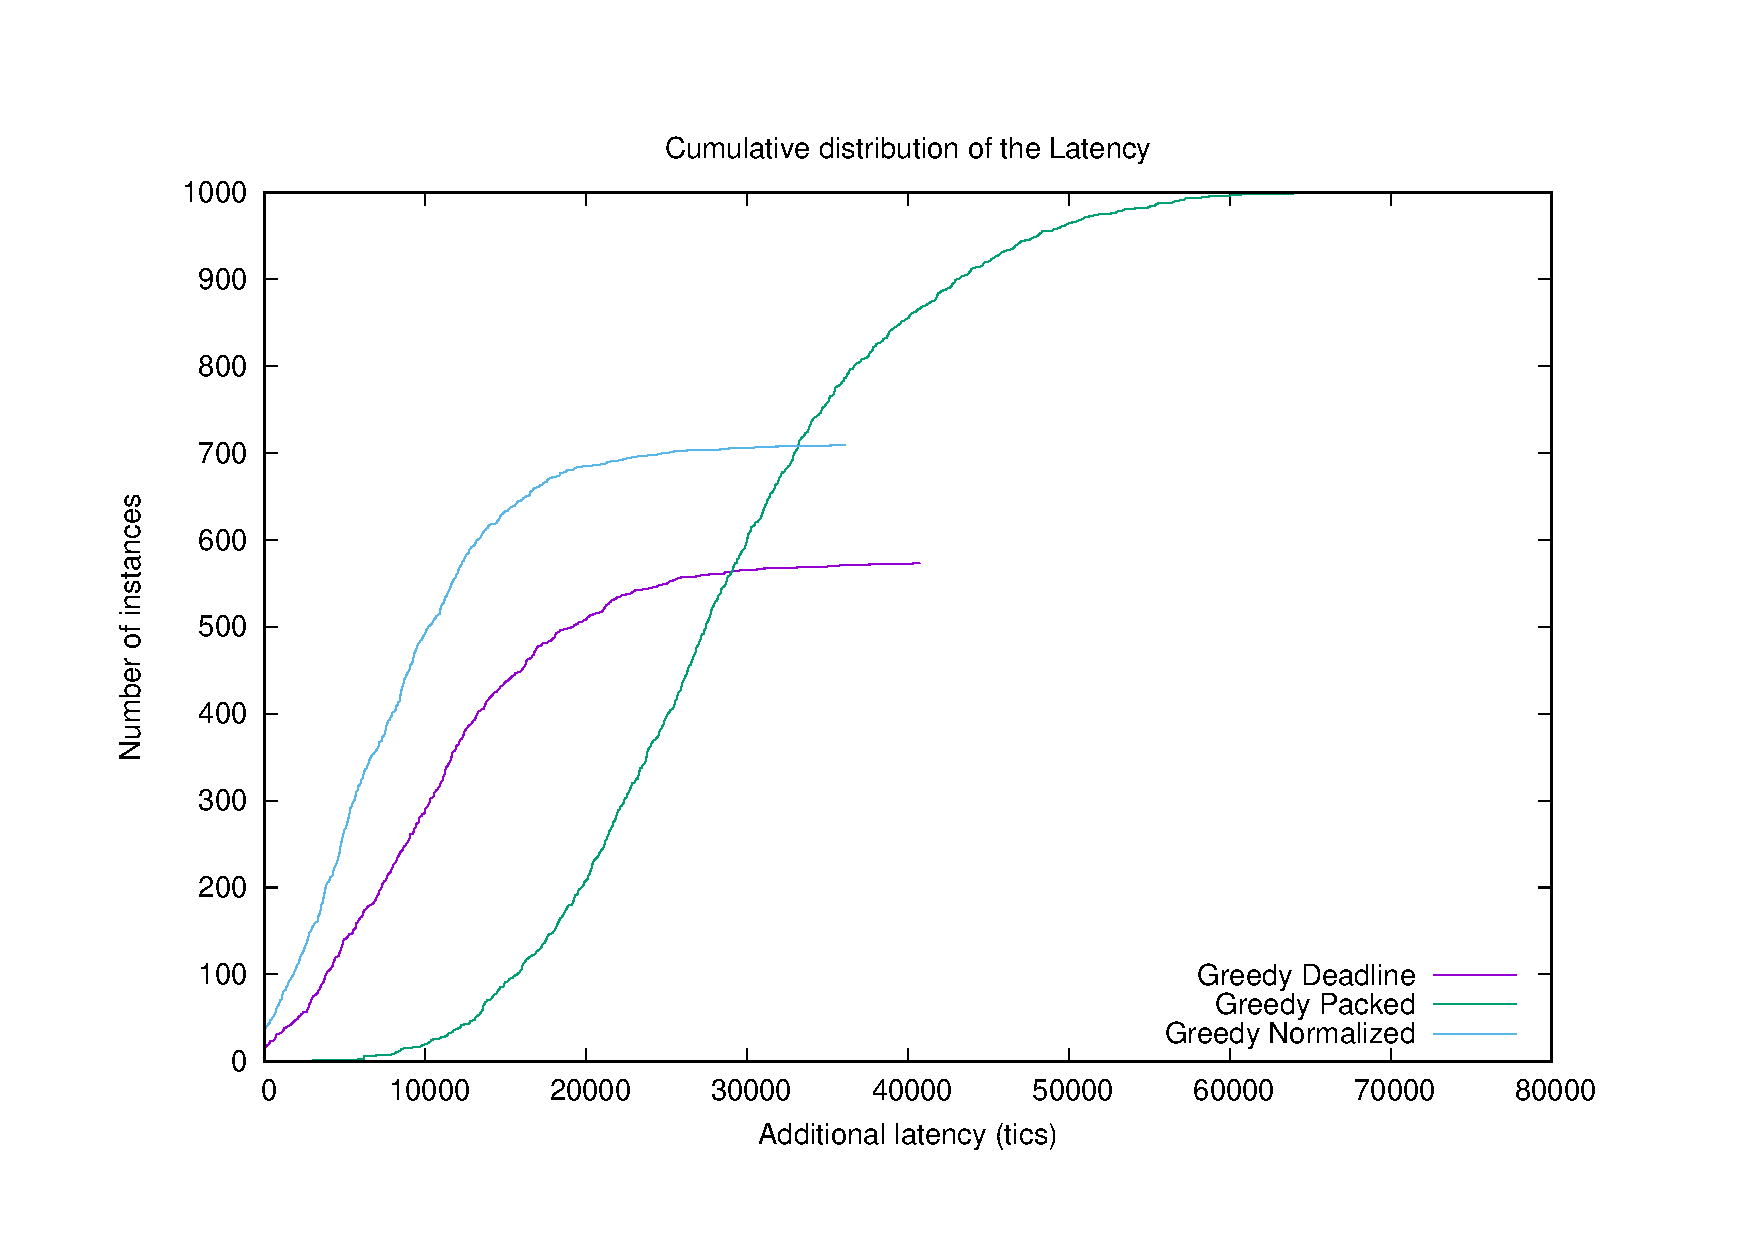
\includegraphics[scale=0.23]{90load}
\captionof{figure}{Performance of \greedydeadline, \greedynormalized and \greedypacked over $1000$ instances on graphs with $90\%$ load.}
\label{fig:90load}
\end{minipage}
\begin{minipage}[c]{.45\linewidth}
	\centering
	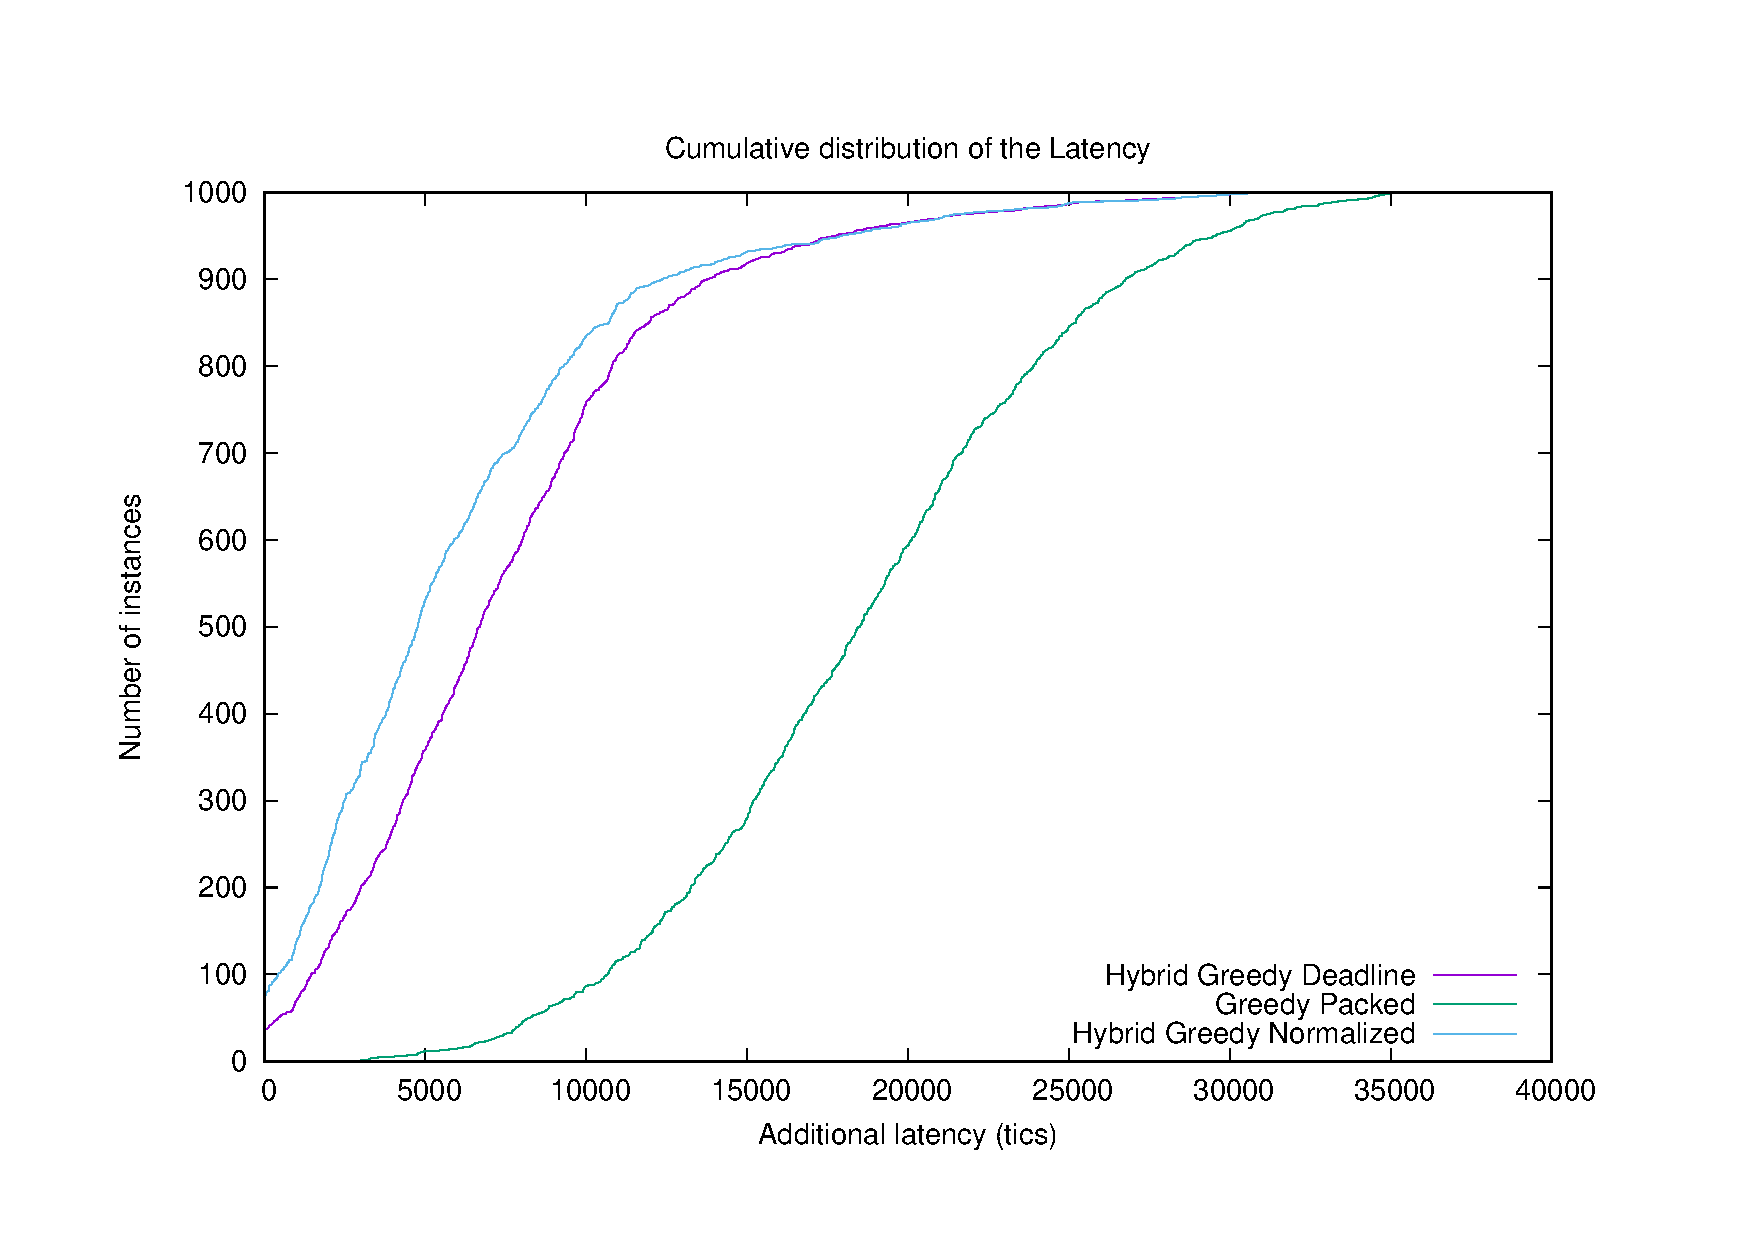
\includegraphics[scale=0.23]{greedysuccess}
\captionof{figure}{ Performance of the updated greedy algorithms that always gives an assignment} 
\label{fig:greedysuccess}
\end{minipage}

Algorithm \hybridgreedynormalized seems much better than the other two. Hence, in the rest of the paper \hybridgreedynormalized will serve 
as a baseline of assignment quality since it can be obtained in very short time. It will also serve to initialize 
local search algorithms with a first assignment of sufficient quality.

\section{Local Search Heuristics}

The number of compact representations grows extremely quickly with $n$. Hence, to find one which minimizes $TR(A)$, we propose several classical local search algorithm: hill climbing, tabu search and simulated annealing. These methods works as long as a relevant notion of neighborood of a solution is proposed. The neighborood relation must satisfy two properties: it must be quick to compute (hence not to large) and the implicit graph of solutions defined
by the neighborood relation should be connected. We now propose a simple neighborood relation over compact assignments.

Let $u$ be a contention vertex of a network, and let $CA$ be a compact assignment for this network, 
 which associates the pair $(O_u,S_u)$ to $u$. Let $O_u = (r_1,\dots,r_l)$.
  Let $r_i \in \mathcal{R}_u$, the \emph{$r_i$-neighborood} of $(O_u,S_u)$ is the set of pairs $(O,S)$ such that:
 
 \begin{enumerate} 
 \item $O = O_u$ and $S_u = S$ or $S \triangle \{r_i\}$  
 \item $O = (r_1,\dots,r_{i-2},r_{i},r_{i-1},\dots,r_{l})$ and $S_u = S$ or $S \triangle \{r_i\}$ or  $S \triangle \{r_{i-1}\}$ or $S \triangle \{r_i,r_{i-1}\}$ 
 \end{enumerate}

Informally, a compact representation is in the $r$-neighborood of another one if it can be obtained by 
moving down $r$ once (or not changing it) in the order and adding or removing $r$ and the previous route from the set. 
Remark that the $r$-neighborood of any pair $(O_u,S_u)$ has at most $6$ members (it can be $4$ when the route $r$ is in first position and cannot be exchanged with the previous one). 

The \emph{$r$-neighborood} of a compact assignment $CA$ is the set of all compact assignments $CA'=(O'_u,S'_u)_{u \in V(G)}$, such that  $(O'_u,S'_u)$ is in the $r$-neighborood of $(O_u,S_u)$. Finally, the \emph{neighborood} of an assignment $CA$ is the union for all $r \in \cal{R}$ of the $r$-neighboroods of $CA$.

% 
% 
% We define $O(r)$ the position of the route $r$ in an order $O$, and the inverse fuction $O^{-1}(r)$.\\
% We consider a compact represtation $(O_u,S_u)$ on a contention point $u$.
% A \textit{neigbhor order} of  $O$ over a route $r$, is an order $O'$ such that $O'(r) = O(r)+1$ . This means that $O'(j) = O(j),\forall j \notin \{r;O^{-1}(r)+1\}$. Indeed, by definition, $O'(O^{-1}(O(r)+1)) = O(r)$. If $r$ is the last route in the order $O$, then $O'(r) = 1$ and $O'(O^{-1}(O(1))=O(r)$
% A \textit{neigbhor subset} of $S$ over a route $r$ is defined by $S' = S - \{r\}$ if $r\in S$ or $S'= S \cup \{r\}$ if $ r \notin S$.
% The \textbf{neighborhood of the pair} $(O_u,S_u)$ ouver a route $r$ is defined by the set $N_u = \{(O_u,S_u);(O_u,S_u');(O_u',S_u);(O_u',S_u')\}$.\\
% 
% Consider a compact representation $CR(A)$ over a route $r$.
% $CR'(A)$ si a \textbf{neighbor} of $CR(A)$ if for all pair $(O_u,S_u)'$ of $CR'(A)$:
% \begin{itemize}
%  \item If $u \notin r$, $(O_u,S_u)' = (O_u,S_u)$
%  \item If $u \in r$, $(O_u,S_u)' \in N_u $
% \end{itemize}
% 
% The \textbf{neighborhood of a compact representation} $CR$ \textbf{over a route} $r$  is thus the set of compact representations: $\prod_{u\in r} N_u$.
% 
% The \textbf{\underline{neighborhood of a compact representation}} $CR$ is then the set of the compact representations over all routes, that is:
% $$ \bigcup_{r\in{\cal R}} (\prod_{u\in r} N_u ) $$.

 Let us denote by $k_1,\ldots,k_n$ the number of contention vertices on the $n$ routes of 
 a routed network $(G,\cal{R})$. Then, a compact representation has at most $\sum_{i=1}^n 6^{k_i}$ neighbors. Since the networks we consider are of bounded contention depth ($2$ or $3$ in practice), the size of a neighborhood is linear in the number of routes.  We further restrict the notion of neighborood to realizable compact assignments. Indeed, the unrealizable compact assignments do not yield a real assignment, their transmission time is not defined and we cannot use them in our local search algorithms. We call the graph defined by the neighborood relation over realizable compact assignments of a routed network the \textbf{transposition graph} of the routed network. 
  All algorithms presented in this section will do a walk in the transposition graph, trying to find a vertex with optimal
  transmission time. 

\todo{Faire un dessin d'un routed network simple}


\begin{lemma}\label{lemma:path}
There is a path from a realizable compact representation CR, with $CR(u) = (O_u,S_u)$ to $CR'$, such that 
$CR'$ is equal to $CR$ except on $u$ where it is equal to $(O_u,S_u \cup E)$.  
\end{lemma}
\begin{proof}
The path is by adding elements in $E$ one by one. 
 To prove the existence of the path, it is enough to prove that for  $E = \{v\}$. By definition, $(O_u,S_u \cup{v})$ is in the neighborood of $(O_u,S_u)$. However, one should also prove that $CR'$ is realizable.
  Since the order in which the buffers are fixed by the algorithm of $Real$ is the same for $(O_u,S_u)$ and $(O_u,S_u \cup{v})$, it is easy to prove by induction that the normalized sending times of $(O_u,S_u \cup{v})$ are less than the normalized sending times of $(O_u,S_u)$. Thus, $CR$ realizable implies $CR'$ realizable. Indeed, 
a compact assignment is realizable if and only if the last normalized sending time is less than $P - \tau$.
\end{proof}



 \begin{theorem}
 The transposition graph of a routed network is connected.
 \end{theorem}
 \begin{proof}
 For simplicity, we assume that the routed network has a single contention node $u$. Let $(O_u,S_u)$ and $(O'_u,S'_u)$ be two realizable compact assignments, we show there is a path between them. Let $r$ be the first element of 
$O_u$ and let $E = \mathcal{R}_u \setminus \{ r \}$. By Lemma~\ref{lemma:path}, there is a path from 
$(O_u,S_u)$ to $(O_u,E)$. Consider now $O_u''$, the order $O_u'$ whith $r$ placed in first position.
There is a path from $(O_u,E)$ to $(O_u'',E)$. Indeed, any order is realizable, when all elements but the first
are in $E$ because there are no constraints on their normalized sending time. 
Now, let $r'$ be the first element of $O_u'$. By definition, $(O_u',E \triangle \{r,r'\})$ is in the $r'$ neighborood of $(O_u'',E)$. Moreover, $(O_u',E \triangle \{r,r'\})$ is realizable because $E \triangle \{r,r'\}$ is equal to all routes but the first in $O_u'$. 
Finally, using Lemma~\ref{lemma:path} once again prove there is a path between $(O_u',E \triangle \{r,r'\})$ and $(O'_u,S'_u)$ since $(O'_u,S'_u)$ is realizable and $S'_u \subseteq E \triangle \{r,r'\}$, which proves the theorem.
 \end{proof}




\subsection{Hill Climbing}

The most simple local search heuristic is hill climbing. This algorithm starts from a compact assignment $CA$, explore the entire neighborhood of $CA$, and select the realizable compact assignment $CA'$ of minimal transmission time. Then, we set $CA = CA'$ and repeat this step until there are no $CA'$ such that $TR(CA') < TR(CA)$. Then algorithm stops and returns $Real(CA)$ which is a local minimum. 

The quality of hill climbing depends of the the intial compact assignment. A first natural intialisation is to consider the compact representation $CR(A)$ of the assignment $A$ given by \hybridgreedynormalized. Also, a random compact assignment can be taken. Since a compact assignment does not always give a valid assignment, the last idea is to execetue several hill climbing starting from a random compact assignment, and to return the best assignment given.

Figure~\ref{fig:descente07} shows the difference between initalizing the hill climbing with \hybridgreedynormalized, or with one or several random compact representation. Those resultas are drawn on $1000$ random instances, with $80\%$ of load.
\begin{figure}[h] 
	\centering
	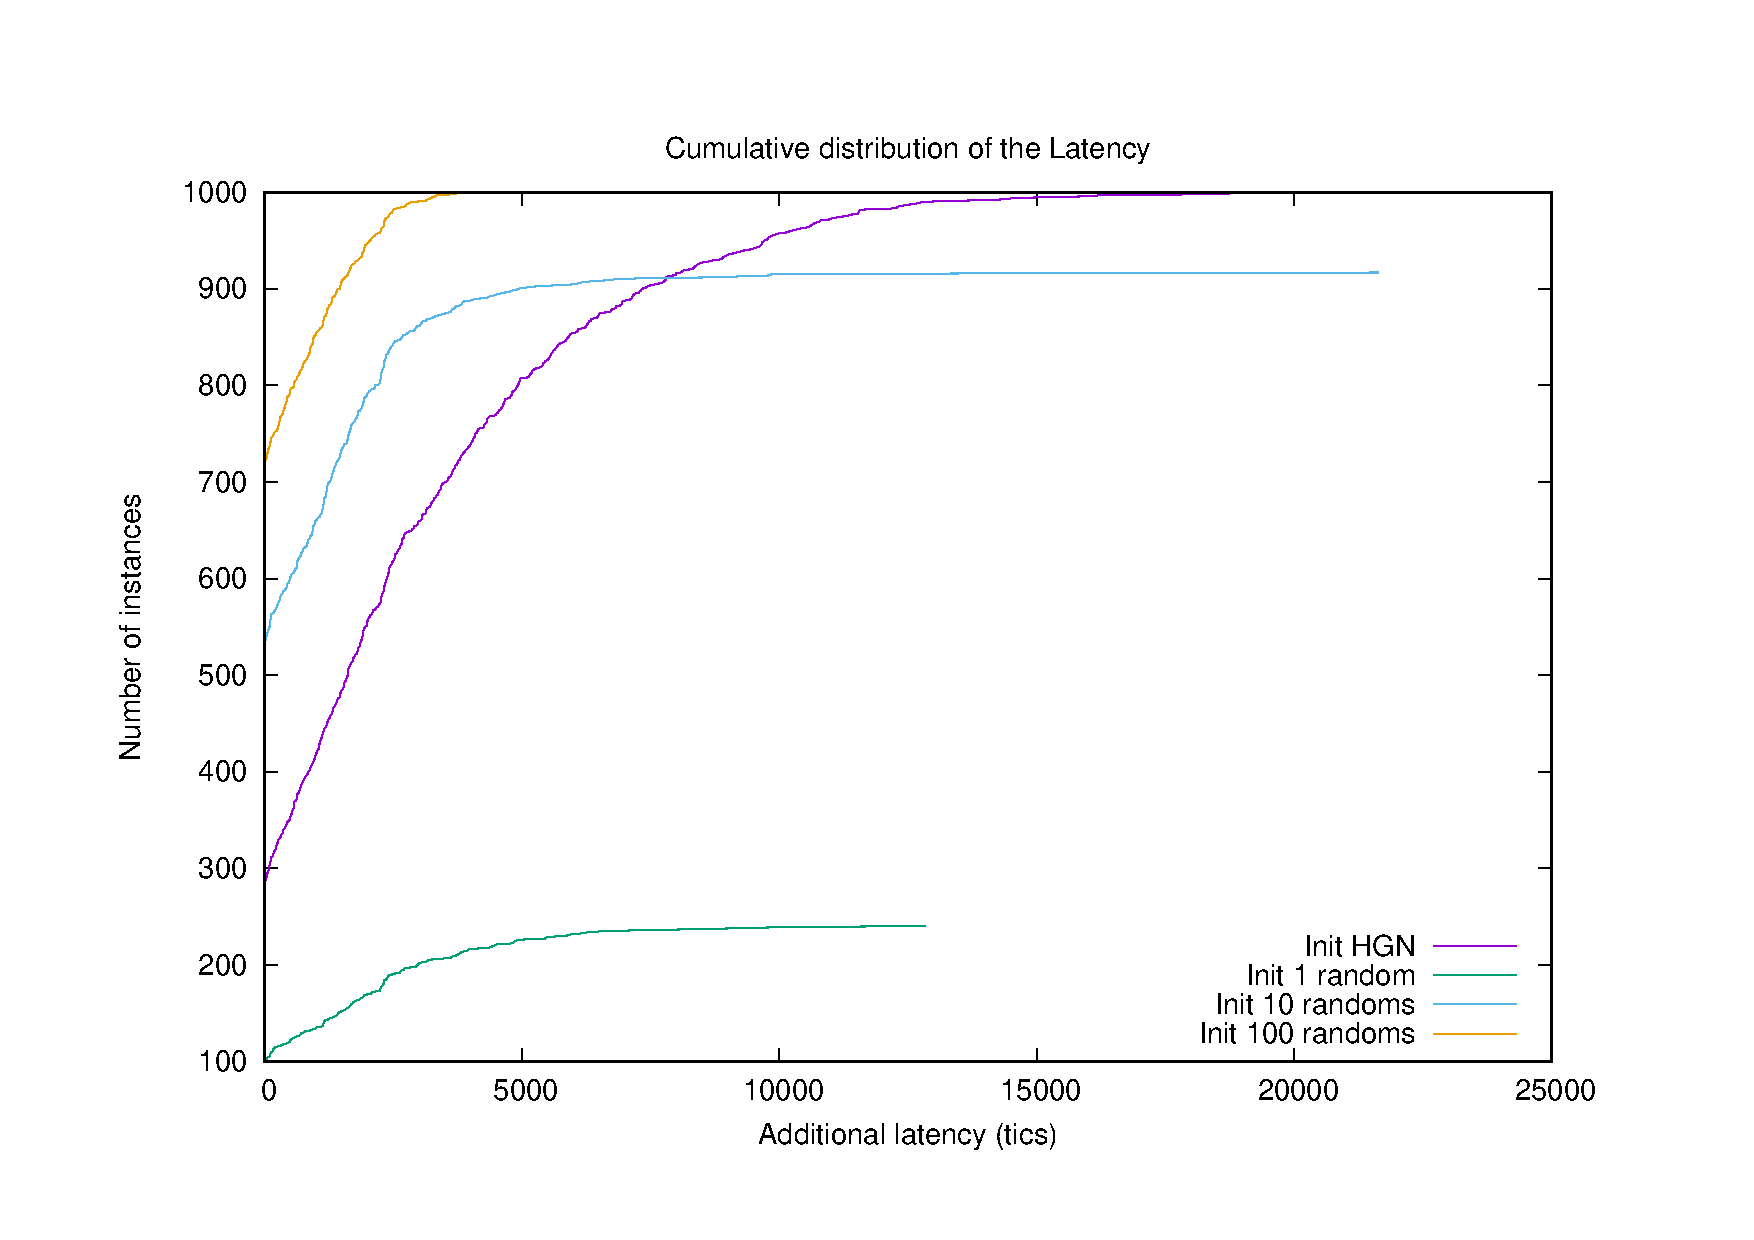
\includegraphics[scale=0.3]{descente07}
\caption{ Additional latency needed to find a solution for hill climbing, intialized with HGN, 1,10 or 100 random compact representation.}
\label{fig:descente07}
\end{figure}
Initializing the hill climbing with 100 randoms compact representation seems to give better results. Nevertheless remember that the set of compact representation does not always give a valid assignment. Drawing some random compact representation can be a limited option when the set of compact representation grows, because the chance of drawing a non valid, or bad random compact representation grows too.

Figures~\ref{tab:descenteload} and \ref{tab:descentenbroutes} represent the probability of drawing at least one compact representation that gives a valid assignment, when drawing $1$,$10$ or $100$ random compact representations. Each result is computed on $1000$ random instances.

\begin{minipage}[c]{.45\linewidth}
\vspace{-0.4cm}
\begin{tabular}{ |c|c|c|c|c| }
\hline
    Load & $80\%$& $90\%$ & $100\%$\\
    \hline
    HGN & $100\%$ & $100\%$& $100\%$ \\
    1 rand & $7\%$ & $4\%$& $6\%$\\
   10 rand & $49\%$& $42\%$& $28\%$\\
   100 rand & $100\%$ & $97\%$& $92\%$\\
    \hline
 \end{tabular}
   \captionof{figure}{Success rate of hill climbing with different initialization, varying the load.}
 \label{tab:descenteload}
\vfill
 \end{minipage}
 \hfill
\begin{minipage}[c]{.45\linewidth}
\vfill
\begin{tabular}{ |c|c|c|c|c| }
\hline
    Nb routes & $8$& $10$ & $12$\\
    \hline
    HGN & $100\%$ & $100\%$& $100\%$ \\
    1 rand & $7\%$ & $2\%$& $1\%$\\
   10 rand & $49\%$& $23\%$& $5\%$\\
   100 rand & $100\%$ & $86\%$& $56\%$\\
    \hline
 \end{tabular}
 \captionof{figure}{Success rate of hill climbing with different initialization, varying the number of routes on the graph.}
 \label{tab:descentenbroutes}
\vfill
\end{minipage}

Those experiences shows that, even if initializing the hill climbing with $100$ random instances performs well when the number of routes and the load are low, this initialization is not robust when the load of the number of routes increases. Indeed, higher loads induces that good solutions are harder to find, and increasing the number of routes also increase the size of the neighboorhood, and thus, the number of non valid compact representations. Furthermore, the computation time induced by executing the hill climbing on a lot of random compact representation instead of only one (for HGN) makes it less effective.


We thus propose an hybrid initialization of hill climbing: Between the assigments given by initializing the hill climbing either with HGN, or with $1$,$10$ or $100$ random compact representation, return the one that minimize $TR(A)$. We call this initialization respectively hybrid $1$, hybrid $10$ or hybrid $100$.
Figure~\ref{fig:hybridhill} shows the additional latency needed by the best solution given by hill climbing, with different initialisations. The results are computed on $1000$ random instances.
\begin{figure}[h]
	\centering
	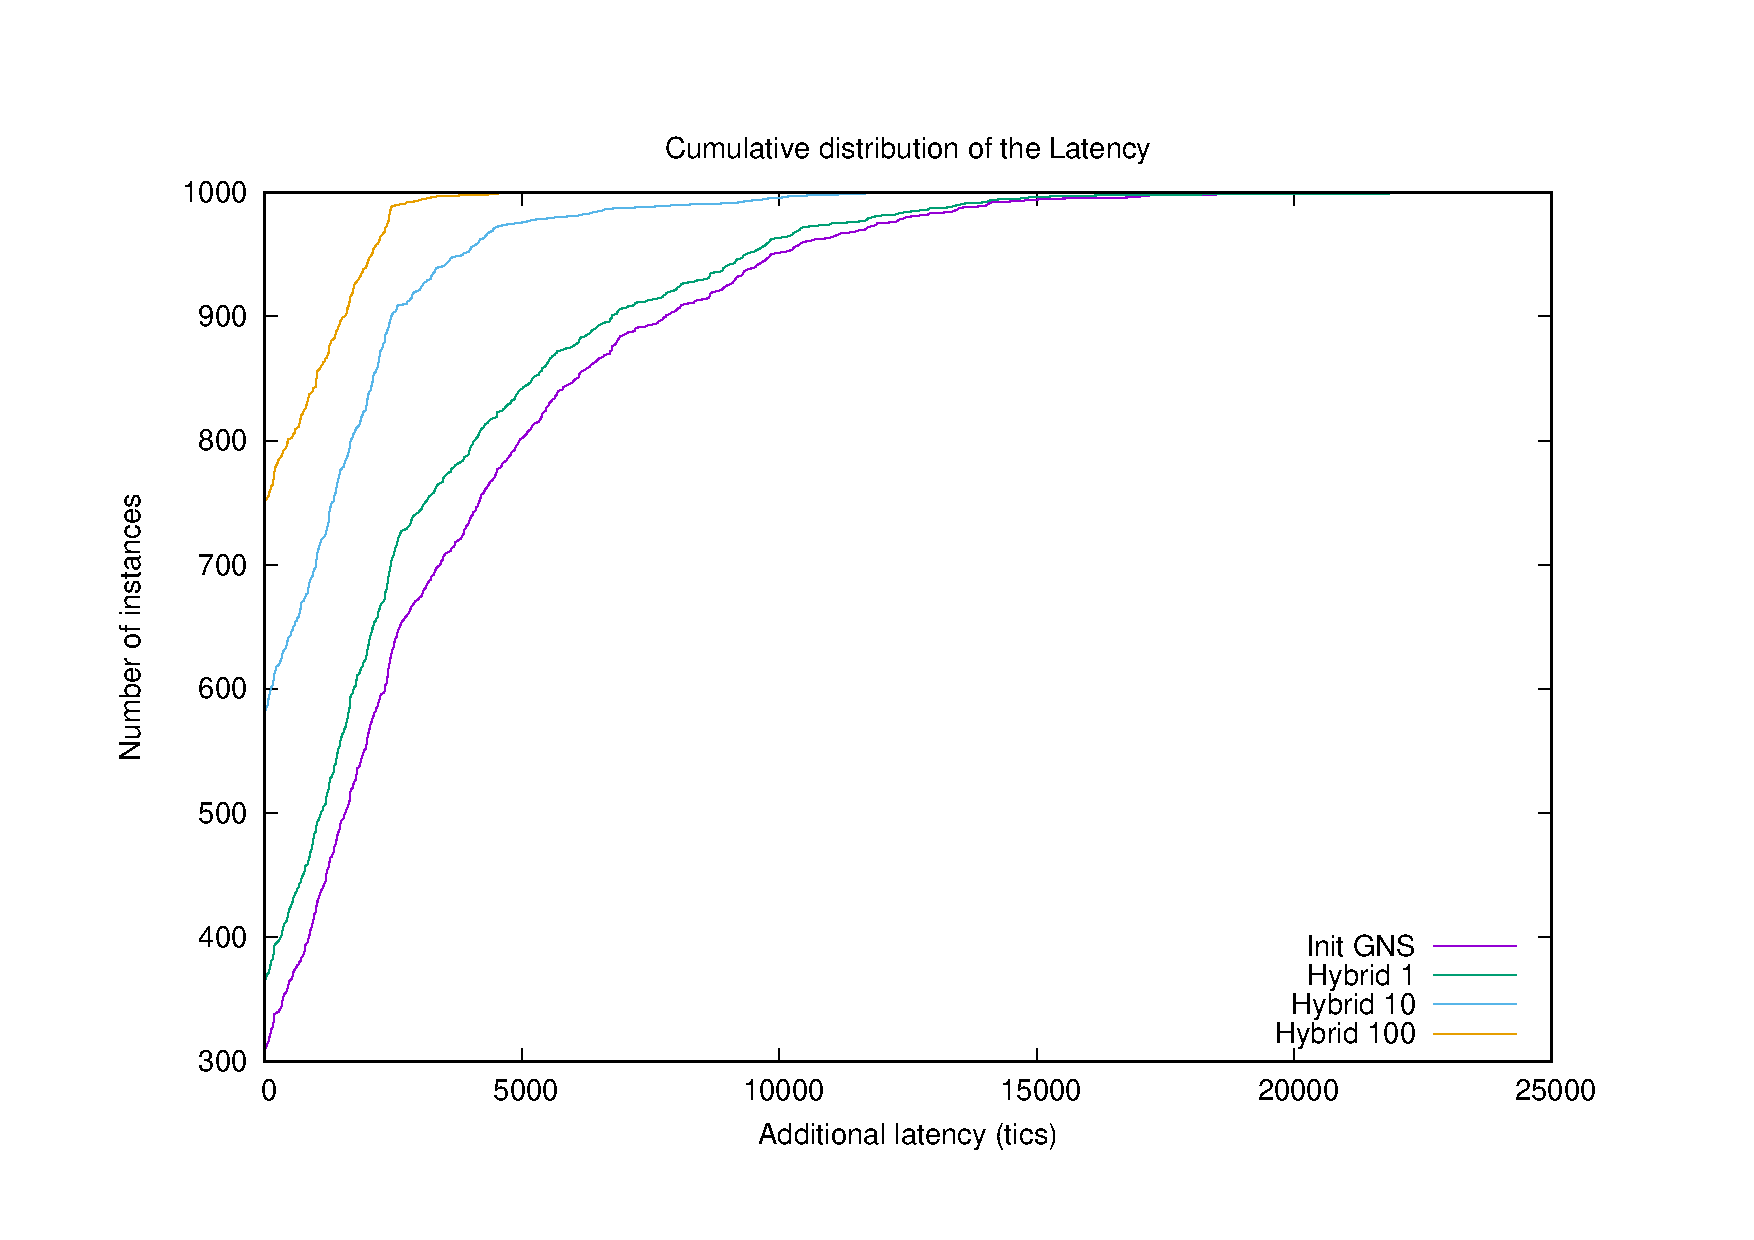
\includegraphics[scale=0.3]{hybridhill}
\caption{ Additional latency needed to find a solution for hill climbing, intialized with HGN, hybrid $1$, hybrid $10$ or hybrid $100$.}
\label{fig:hybridhill}
\end{figure}

We now focus on how many steps hill climbing computes before ending. Tabular~\ref{tab:nbstepdescente} shows the average number of steps of the hill climbing with different initializations. Those results come from the experiment of figure~\ref{fig:hybridhill}.

\begin{tabular}{ |c|c|c|c|c| }
\hline
    Init & HGN& Hybrid $1$& Hybrid $10$& Hybrid $100$\\
    \hline
    Average Nb Step & $1.14$ & $1.26$& $1.92$&$3.38$ \\

    \hline
 \end{tabular}
  \captionof{figure}{Average number of step needed by hill climbing to reach a local optimum.}
 \label{tab:nbstepdescente}

 The more the hill climbing does steps before ending, the more the initial solution is improoved. When hill climbing starts from a \hybridgreedynormalized, it does not improove often the solution whereas with a huge number of random compact representation, the probability of drawing a solution that can be improoved a lot is increased.
 
 The concept of drawing a large number of random compact representation to initialize the hill climbing link with the concepts of taboo search and simulated annealing. Indeed, the two next meta-heuristics are designed to explore the compact representations, even if a local optimum is reached. Taboo remembers the explored solutions, in order to avoid it, and simulated annealing browse the compact representations with a stochastic aspect.
\subsection{Tabu Search}

Tabu search is a variation on hill climbing using memory. We also select the compact assignment $CA'$ which minimizes 
$TR(CA')$, even when $TR(CA') < TR(CA)$ is not satisfied. To avoid loop in local minimum, we use a memory of the last 
$N$ solutions explored and we forbid to visit them again. This algorithm can still loop on a cycle larger than $N$,
hence we must fix some integer $M$ and stop the algorithm after $M$ steps.


One can change the size $N$ and $M$ in tabu search -> explore how to fix these parameters. 

After reaching a local optimum, tabu search continues it execution untill it has executed a given number of steps.
Thus, we investigate the average number of steps needed by the tabu search to find the assignment it returns. Remember that, to each step, the search explores the entire neighborhood of a solution. The computation of a large number of steps is then long.

Tabu search has a memory, it remembers the compact assignment for which it explored the neighborhood for the $x$ last solutions in order to not visit them again. Varying the value of $x$ can improve or worsen the performance of the tabu search.
Figure~\ref{fig:tabudistrib} shows cumulative distribution of the additional latency needed by tabu search with different size of memory. The number of steps computed by the tabu search is $1000$.
\begin{figure}[h]
	\centering
	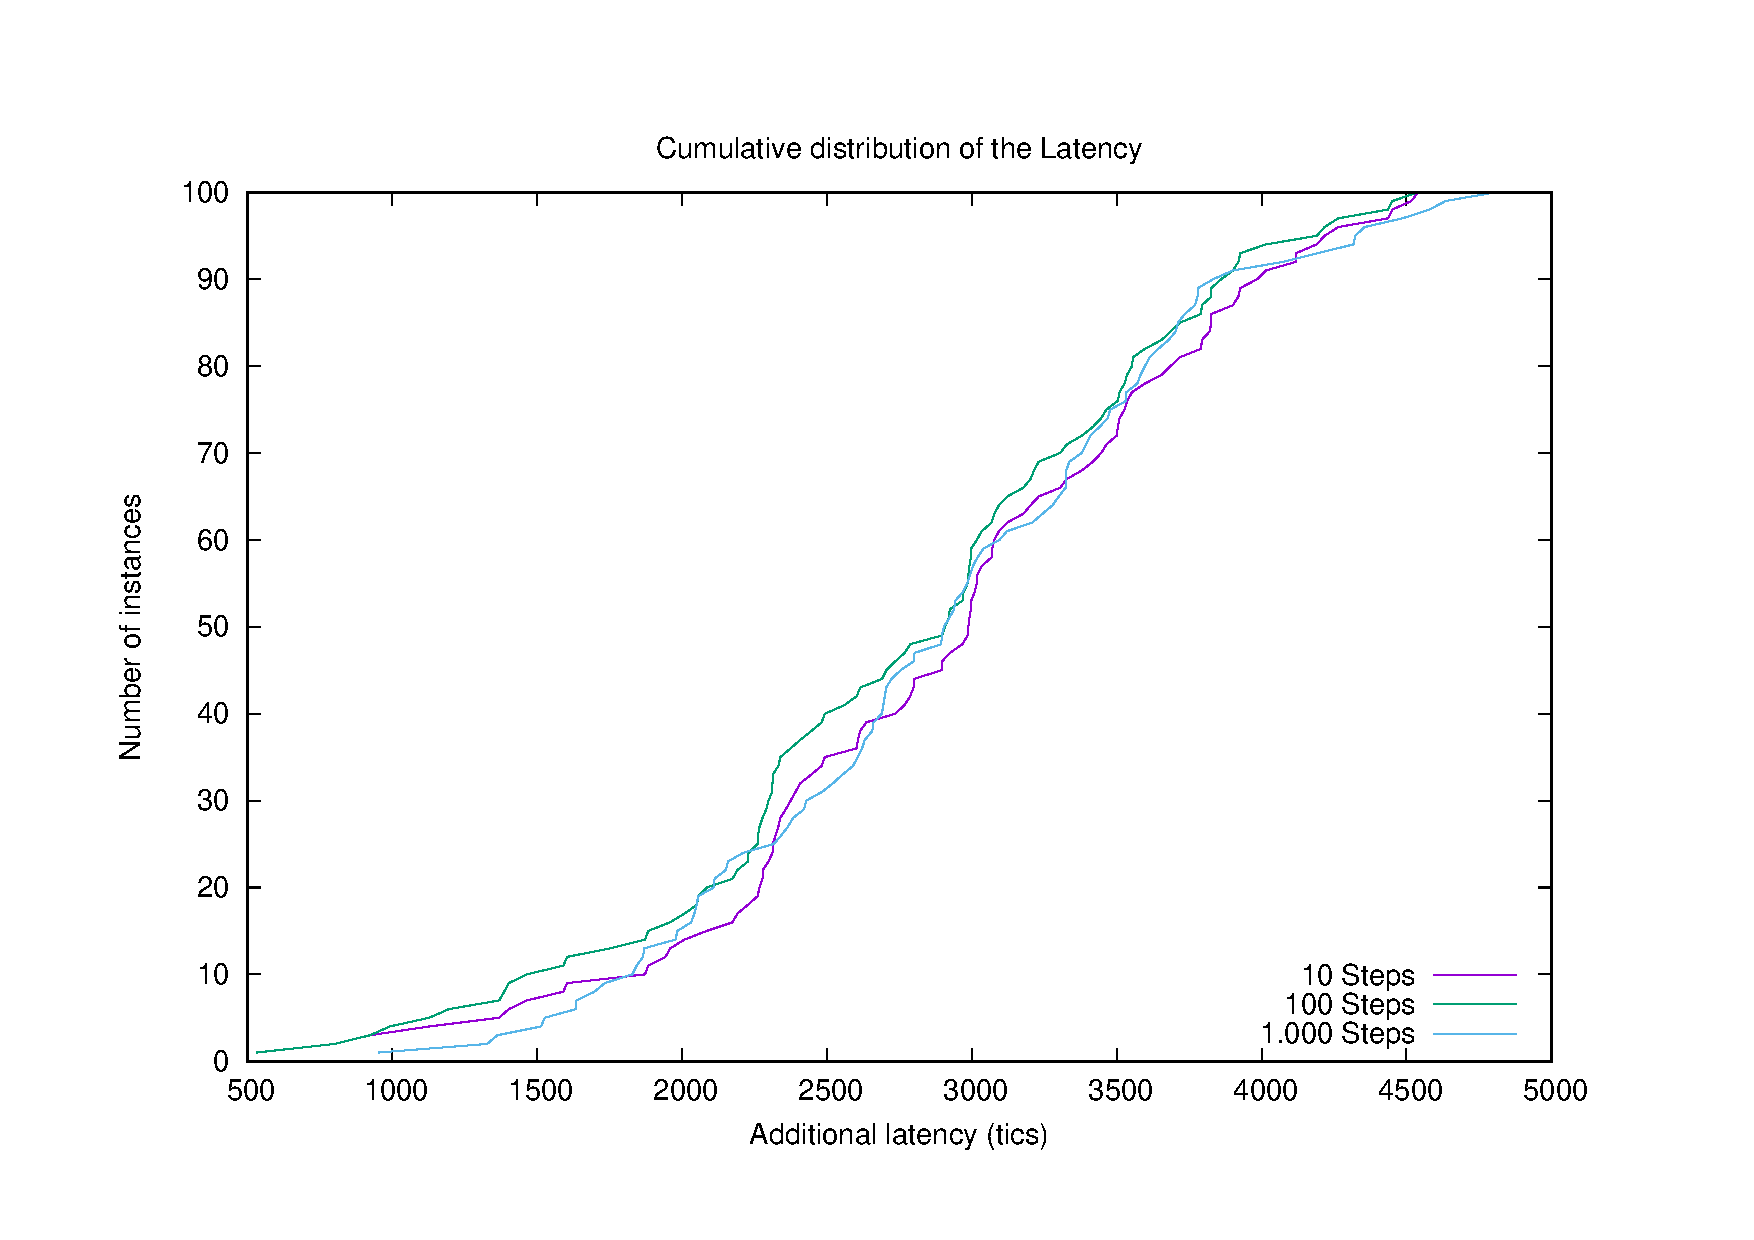
\includegraphics[scale=0.3]{taboo_distrib}
\caption{ Difference between the tabu search whith a memory of $10$,$100$ or $1000$ solutions}
\label{fig:tabudistrib}
\end{figure}
It appears that, the more steps tabu search remember, the better the assignment given is.
In order to understand what happends during the tabu search, we investigate the distribution of the step at which the tabu search finds its best solution.
For $10$ steps of memory, tabu search finds the best assignment in average in $3.8$ steps, with a memory of $100$ steps, the average step that gives the best assignment is $18.1$, and for $1000$ steps, tabu search needs in average $84.3$ steps to find the best solution. 
Also, it appears that, in most of $60\%$ of the cases, tabu search finds it's best assignment before $10$ steps, but some computation finds a better assignment up to the $900^{th}$ step. This means that running the tabu search longer could improove the quality of the result. Nevertheless, this the computation is really expensive, using simulated annealing is more interesting.

\subsection{Simulated annealing}

A simulated annealing search works as follow. A {\emph temperature} is set. Considering a compact assignment $CA$, we draw in its neighborhood a compact assignment $CA'$. Then, considering the temperature, $TR(Real(CA))$ and $TR(Real(CA'))$, the compact assignment $CA'$ is or accepeted or rejected. If it is accepted, the neighborhood of $CA'$ is then explored. During the simulated annealing, the temperature decrease. The lower is the temperature, the lower are the chance to accept a compact assignment that worsen the solution.

 Simulated annealing needs two parameters to run. A temperature, and a number of steps.
 The temperature must be fixed in order to accept to worsen the solution at the begining of the execution, must decrease slowly. When the temperature is low, the simulated annealing rejects bad compact representations.
 Accepting or rejecting a solution is a stochastic process. Consider $CA$, the best compact assignment found during the exection of the simulated annealing. The value $\Delta$ represent the difference $TR(REAL(CA'))-TR(REAL(CA))$ where $CA'$ is a compact assignment in the neighboorhood of $CA$. $CA'$ is accepted or rejected with the probability $e^{-\frac{\Delta}{t}} $, where $t$ is the temperature.
 This means that $\frac{\Delta}{t}$ must be close to $0$ at the begining, and must approaches infinity at the end of the execution. 
 
 In order to fix the initial temperature $t_0$, we compute a routine explained in \cite{osman1997meta}:
 \begin{enumerate}
  \item Initiate 100 disturbances at random; evaluate the average $\bar{\Delta}$ of the corresponding variations $\Delta$
\item Choose an initial rate of acceptance $\tau_0$ of the “degrading perturbations” according to the assumed “quality” of the initial configuration; for example:
\begin{itemize}
 \item “poor” quality: $\tau_0 = 50 \%$ (starting at high temperature)
\item “good” quality: $\tau_0 = 20 \%$ (starting at low temperature)
\end{itemize}


\item Deduce $t_0$ from the relation: $e^{-\frac{\bar{\Delta}}{t_0}} = \tau_0$ 
 \end{enumerate}
 
 Tabular~\ref{tab:poorgood} shows the additional latency needed by simulated annealing when intialized with two intial temperatures computed from the previous routine. The first solution considered by simulated annealing is the solution given by hill climbing. The experiment is made over $100$ instances. During the computations $1000$ compact representation are drawn before decreasing the temperature.
\begin{center}
\begin{tabular}{ |c|c|c|c|c| }
\hline
 Quality of initial configuration & Good& Poor\\
    \hline
    $t_0$ & $2200$& $13000$\\
    \hline
    Additional latency & $4212$ & $4217$ \\
        \hline
    Computation time (ms) &  $2.817$&$4.035$ \\

    \hline
    
 \end{tabular}
 \caption{Comparison of two intial temperatures, considering the quality of the initial configuration}
     \label{tab:poorgood}
 \end{center}
 As observed, the initial solution given by hill climbing can be considered as ``good''. Indeed, increasing the initial temperature does not affect the quality of the solution, but increase the computation time.
 
 In simulated annealing, the temperature decrease slowly. Each \textbf{level}, several compact representation are drawn. At the end of a level, the temperature is decreased. Drawing too few compact representation per level induce decrasing the temperature too fast and thus, reducing the efficiency of simulated annealing. In an ohter hand, drawing too much compact representation increases the computation time of the algorithm.
 
 We investiage the impact of drawing a large number of compact representation before decreasing the temperature. Figure~\ref{fig:stepsrecuit} shows the additional latency needed by simulated annealing with different number of compact representation draw for each level. Those results comes from $100$ random instances, in which the temperature is set to $2200$.
 
 \begin{figure}[h]
	\centering
	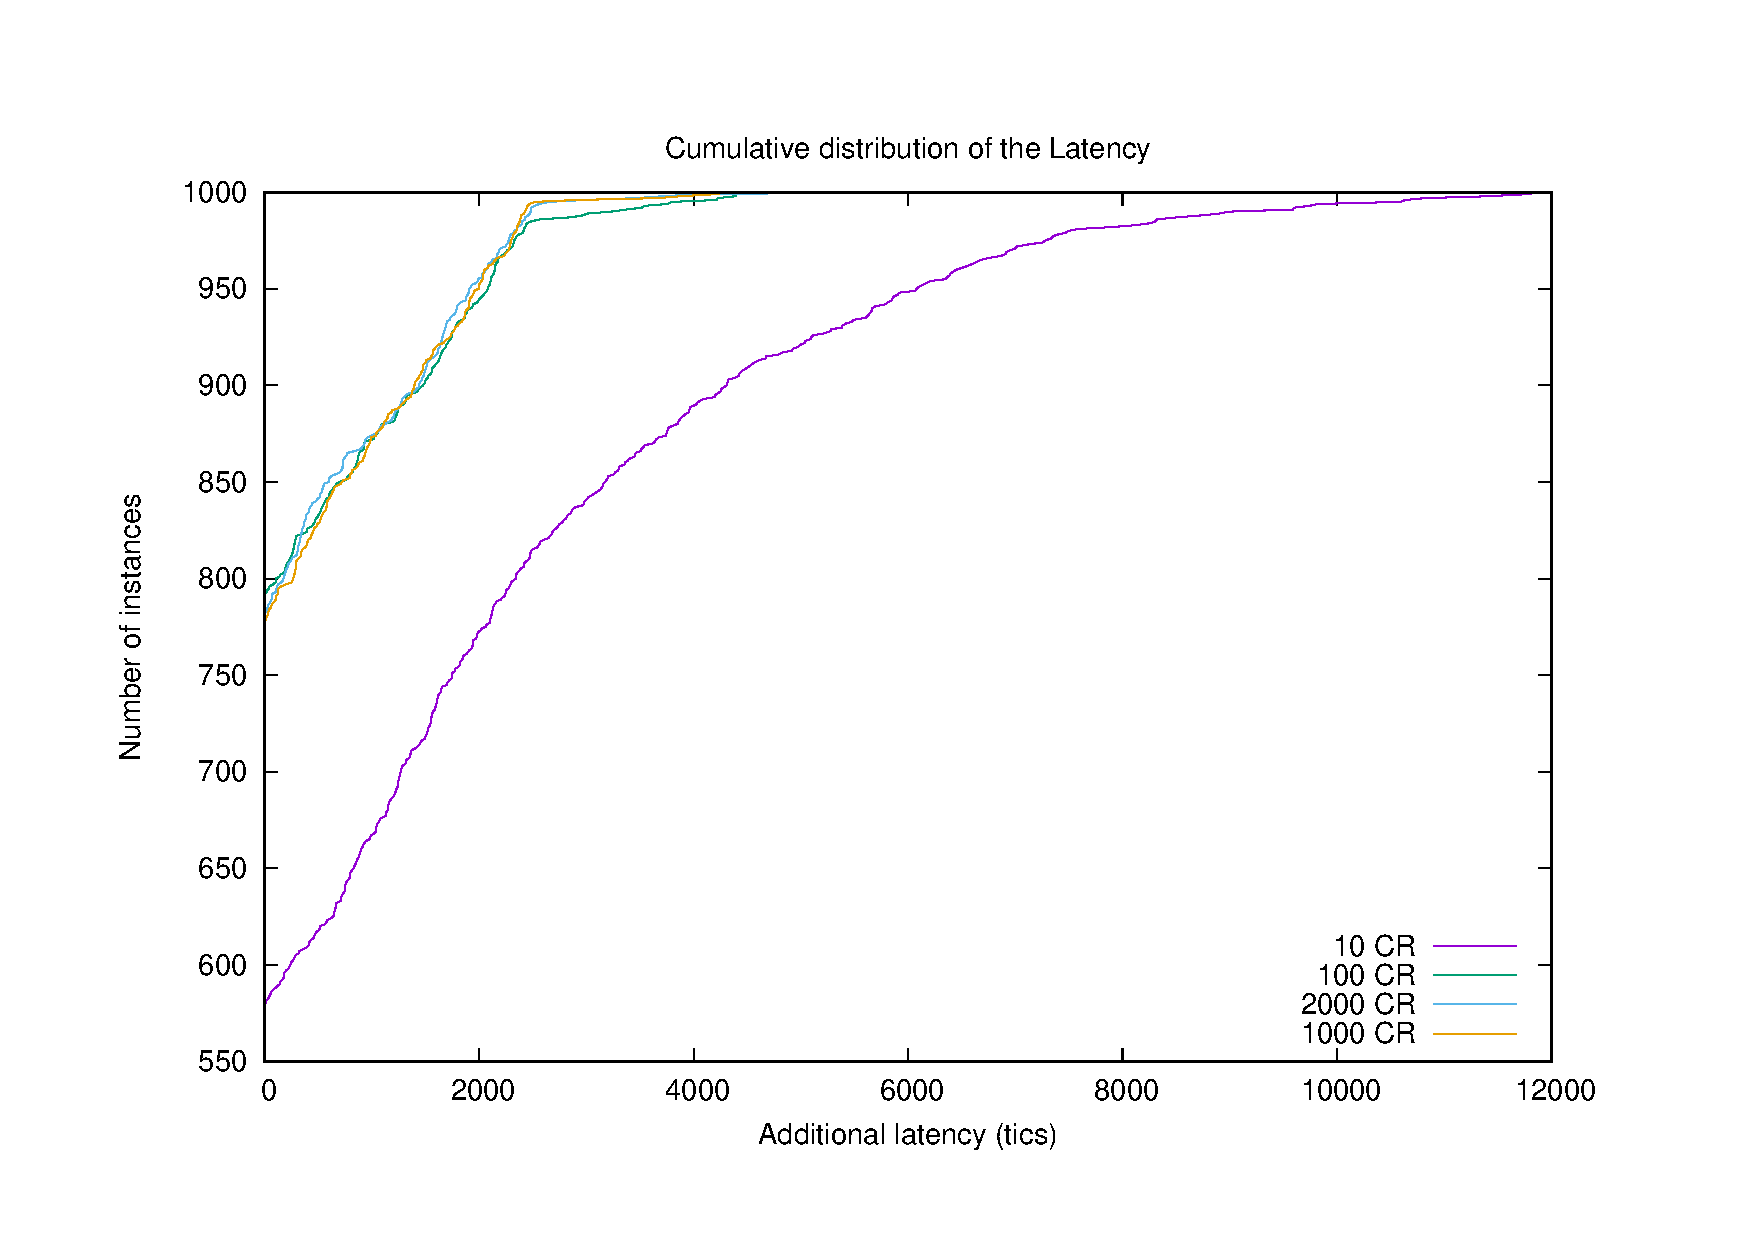
\includegraphics[scale=0.4]{stepsrecuit}
\caption{ Additional latency needed to find a solution for simulated annealing, with a different number of compact representation drawn to each level.}
\label{fig:stepsrecuit}
\end{figure}
It appears that drawing more than $1000$ compact representation per level does not improove the quality of the solution, while it increase the computation time.

\todo{differents profils de temperature}


\subsection{Branch and Bound}

D'abor introduire la notion de solution partielle (avec seulement une partie des temps d'attente fixée).
Puis définir le graphe associé à une solution partielle (en enlevant les sommets déjà traités).

Puis donner la relaxation du problème général au problème sur un point de contention. 
Définir la borne inf comme le max de la relaxation pour tous les points de contention.

Définir l'arbre de recherche exhaustif avec coupe grace à la borne inf.

Enfin optimisation: proposer un ensemble de coupes efficaces qui permettent d'oublier la plupart des solutions 
non minimales + traitement spécifique du dernier niveau.

Montrer avec des courbes (nombre de représentation générées et pourcentage de minimales en fonction du nombre de routes) que ces coupes sont très efficace, elles permettent de générer uniquement des représentations compactes canoniques, et presque aucunes dont la réalisation n'est pas minimale.

\subsection{Results comparison}



\section{Autres trucs à raconter}
Once all those synthetic datas are set, we focus on the length of the arcs in the grap. We look at three ways to draw some values for the length of the arcs: uniformly between $0$ and $\tau/3$ (with $\tau$ the size of a datagram), uniformly between $0$ and $P$ (the size of the period), and uniformly between $P-0.1\times P$ and $P$.
\todo{expliquer pourquoi ces valeurs}

Figure~\ref{tab:instances} shows the average additional latency needed by the branch and bound and the greedy algorithm that we call HGN presented in next section (used to intialize the local search algorithms) for the different ways to draw the length of the arcs. Those values are draw for $100$ instances of each kind.

\begin{center}
\begin{figure}
\centering
\begin{tabular}{ |c|c|c|c|c| }
\hline
    Range & $0$ and $\tau/3$ & $0$ and $P$& $P-0.1\times P$ and $P$\\
    \hline
    Branch and bound & $4273$ & $222$& $2704$ \\
 
    HGN & $12177$ & $10628$& $9648$\\
   
    \hline
  
 \end{tabular} 
 \caption{Difference between the optimal solution of the greedy algorithms, for different kind of instances generated.}
 \label{tab:instances}
 \end{figure}
 \end{center}
 The objective is to find the instances in which a solution given can be the most improoved by the local search heuristics. As observed, when drawing the size of the arcs betwenn $0$ and $P$, the lower bound (found by the branch and bound algorithm) is clearly lower than with the other kinds of instances while the additional latency needed by HGN remains in the same order of magnitude.
 
\section{Conclusion}
C'est vraiment génial comme travail, on va tuer le game du DETNET.

\bibliographystyle{ieeetr}
\bibliography{srcs}
\end{document}
